% This is the main file of your thesis. Preambles, necessary command, etc goes here
% File utama tesis. Command penting, pembuka, dll ditaruh disini
% IT IS IMPORTANT TO PUT THIS FILE IN THE SAME DIRECTORY AS thesisitb.sty
% PENTING! TARUH FILE INI PADA DIREKTORI YANG SAMA DENGAN thesisitb.sty
% By: MF/13612020/23616034 & MI/13612038/23616033
% Credits: LaTeX inventor, SPS thesis guide, Google, and tex.stackexchange
% Terima kasih kepada: yang bikin LaTeX, panduan tesis SPS, Google, dan tex.stackexchange

\documentclass[12pt,english]{report}
\usepackage{thesisitb}

% Reducing spacing bw header and chapter title
% Mengurangi spasi antara batas atas kertas dengan judul bab
\makeatletter
\def\@makechapterhead#1{%
  %%%%\vspace*{50\p@}% %%% removed!
  {\parindent \z@ \centering \normalfont
    \ifnum \c@secnumdepth >\m@ne
        \huge\bfseries \@chapapp\space \thechapter
        \par\nobreak
        \vskip 20\p@
    \fi
    \interlinepenalty\@M
    \Huge \bfseries #1\par\nobreak
    \vskip 40\p@
  }}
\def\@makeschapterhead#1{%
  %%%%%\vspace*{50\p@}% %%% removed!
  {\parindent \z@ \centering
    \normalfont
    \interlinepenalty\@M
    \Huge \bfseries  #1\par\nobreak
    \vskip 40\p@
  }}
\makeatother
\begin{document}
\clearpage

\begin{titlepage}
\begin{center}
%\vspace*{0.75cm}

\large
\textbf{EXPERIMENTAL THRUST OPTIMISATION OF A VARIABLE-STIFFNESS FIN PANEL USING GLOBAL SURROGATE-ASSISTED GENETIC ALGORITHM WITH KRIGING}

\vspace{0.25cm}
\normalsize
\textbf{THESIS}\\
\textbf{This thesis is submitted}\\
\textbf{as partial fulfillment for Master degree}\\
\textbf{from Institut Teknologi Bandung}

\vspace{1cm}

\textbf{by}\\
\textbf{Muhammad Iqbal}\\
\textbf{23616033}\\
\textbf{(Aerospace Engineering Programme)}\\

\vspace{2.25cm}

\includegraphics[width=0.20\textwidth]{ITB_S.jpg}
\vspace{1.75cm}

\large
\textbf{Institut Teknologi Bandung}\\
\textbf{2018}

\end{center}
\end{titlepage}
 % Title page / Judul
\pagenumbering{roman} % Use roman numbering style / Gunakan penomoran halaman gaya romawi

% English abstract page. Write your English abstract in misc/abstrak_eng.tex
% Halaman abstrak. Tulis di misc/abstrak_eng.tex
\chapter*{\centering Abstract}
\addcontentsline{toc}{chapter}{Abstract}
\begin{center}{
    \textbf{EXPERIMENTAL THRUST OPTIMISATION OF A VARIABLE-STIFFNESS FIN PANEL USING GLOBAL SURROGATE-ASSISTED GENETIC ALGORITHM WITH KRIGING}\\
    by\\
    \textbf{
        Muhammad Iqbal\\
        23616033\\
        (Aerospace Engineering Programme)
    }
}
\end{center}
This thesis discuss how the flexibility of a variable-stiffness fin panel model affects the generated net thrust. An optimisation algorithm, global surrogate-assisted genetic algorithm with Kriging was used to optimise the net thrust force produced by the fin panel model, where kriging was used to construct a surrogate model to accelerate the optimisation process. Fitness value was evaluated by directly measuring the thrust force in towing tank experiment. Fin panel model was created using silicon rubber embedded with six spring wires. The fin panel's flexibility can be varied by changing the length of six springs embedded within the silicon rubber, which enables the fin panel to have flexibility range of 0.08 GPa to 207 GPa. The data shows that there exist an optimum stiffness condition which holds true for different kinematical parameters variation. However, different stiffness configurations also change the optimum frequency of the fin, with lower frequency fin responds favorably to lower stiffness configuration fin due to different bending response for a given material properties. It is also shown that there exist a more prominent kinematical parameter which produce the larger optimum thrust compared to the other, less sensitive, kinematical parameter.\par
\textit{Keywords: experimental fluid dynamics, genetic algorithm, kriging, surrogate modeling, flapping flexible panel}


% Legalisation page. Write your legalisation in misc/leg_page.tex
\chapter*{\centering Legalisation Page}
\addcontentsline{toc}{chapter}{Legalisation Page}
\begin{center}
  {\normalsize \textbf{EXPERIMENTAL THRUST OPTIMISATION OF A VARIABLE-STIFFNESS FIN PANEL USING GLOBAL SURROGATE-ASSISTED GENETIC ALGORITHM WITH KRIGING}}\\

	\par
	\vspace{0.8cm}
	{by
	\\
	\large \textbf{Muhammad Iqbal}\\
	\large \textbf{23616033}\\
	\large \textbf{Aerospace Engineering Programme}\\
	
	Institut Teknologi Bandung

	}

THESIS APPROVAL\\
This thesis has been approved and legalised as partial fulfillment for Master degree in Aerospace Engineering Programme.

Bandung, 27 September 2018\\[0.2cm]
Approved by:

Advisor: \\[2 cm]

(Dr. Lavi R. Zuhal) 
\end{center}


%\chapter*{\centering Abstrak}
%\addcontentsline{toc}{chapter}{Abstract (Indonesian)}
%\begin{center}{
    \textbf{OPTIMISASI GAYA DORONG DARI SEBUAH PANEL EKOR DENGAN KEKAKUAN BERVARIASI SECARA EKSPERIMENTAL MENGGUNAKAN \textit{GLOBAL SURROGATE-ASSISTED GENETIC ALGORITHM} DAN \textit{KRIGING}}\\
    oleh\\
    \textbf{
        Muhammad Iqbal\\
        23616033\\
        (Program Studi Teknik Dirgantara)
    }
}
\end{center}
Tesis ini mendiskusikan tentang pengaruh kekakuan pada sebuah panel ekor dengan kekakuan yang variatif pada gaya dorong total yang dihasilkan oleh panel tersebut. Sebuah algoritma optimisasi, \textit{global surrogate-assisted genetic algorithm} dengan \textit{kriging} digunakan untuk mengoptimalkan gaya dorong total yang dihasilkan oleh model ekor, dimana \textit{kriging} digunakan untuk membentuk sebuah model pengganti sehingga proses optimisasi dapat dipercepat. Nilai \textit{fitness} dievaluasi dengan melakukan pengukuran gaya dorong secara langsung pada eksperimen \textit{towing tank}. Model panel ekor dibuat dari karet silikon yang didalamnya terdapat enam buah kawat pegas baja. Kekakuan dari model tersebut dapat divariasikan dengan mengubah panjang dari enam buah kawat tesebut, sehingga panel ekor tersebut memiliki kekakuan dari 5.5 MPa hingga 200 GPa. Data yang didapat menunjukkan bahwa ada sebuah kondisi kekakuan optimum yang menghasilkan gaya dorong total yang paling besar. Kondisi kekakuan ini tetap berlaku untuk kondisi parameter kinematika yang berbeda-beda. Namun, konfigurasi kekakuan panel ekor juga berubah apabila frekuensi dari gerakan mengepak ekor tersebut juga berubah, dengan frekuensi kepak yang rendah membutuhkan kekakuan yang rendah pula untuk menghasilkan gaya dorong total yang paling optimum. Disajukan pula bahwa ada sebuah parameter kekakuan yang lebih berpengaruh pada pembangkitan gaya dorong total yang optimal apabila dibandingkan dengan parameter kinematika lainnya.\par
\textit{Kata kunci: dinamika fluida eksperimental, algoritma genetik, \textit{kriging}, model pengganti, panel fleksibel}

% Preface chapter. Write your preface in misc/preface.tex
\chapter*{\centering Thesis User Guide}
\addcontentsline{toc}{chapter}{Thesis User Guide}
This master degree thesis is registered and available in the library of Institut Teknologi Bandung (ITB) and is open for public with copyright on the author and by following the rules of intellectual property rights in Institut Teknologi Bandung (ITB). Literature references are allowed to be recorded but citations are only allowed with permission from the author.\par
The citation to this thesis in Indonesian can be written as follows:

Iqbal, M. (2018): \textit{Optimisasi gaya dorong eksperimental sebuah panel ekor dengan kekakuan bervariasi menggunakan global surrogate-assisted genetic algorithm dengan kriging}, Tesis Program Magister, Institut Teknologi Bandung.

and in English as follows:

Iqbal, M. (2018): \textit{Experimental thrust optimization of a variable-stiffness fin panel using global surrogate-assisted genetic algorithm with kriging}, Master's Program Thesis, Institut Teknologi Bandung.

To copy or to publish a part or the entirety of this thesis is only allowed with the permission from Director of Graduate School, Institut Teknologi Bandung.

This thesis was written using LaTeX, a part of TeX project.

% Acknowledgement page. Write your acknowledgement page in misc/kata_pengantar.tex
\chapter*{\centering Acknowledgement}
\addcontentsline{toc}{chapter}{Acknowledgement}
James Gleick said that an experimenter has to muster graduate students, cajole machinists, and flatter lab assistants. I would like to dedicate this section to those who I flatter, cajole, and muster in order to complete my thesis.\par
My utmost gratitude obviously goes to The Creator and two of His: my parents. Their love and support for me has been without equal, and this thesis is, in a way, an expression of my gratitude and respect for them.\par
My academic life would be unnecessarily difficult if not for the assistance from my advisors and lecturers: Dr. Lavi R. Zuhal for his guidance on my thesis and life in general and Prof. Tatacipta Dirgantara for his insight on the structural matters on my thesis. Dr. Rianto A. Sasongko for trusting me to tutor students in Engineering and Advanced Mathematics. Also my thesis examiners Dr. Djoko Sardjadi and Dr. Firman Hartono for their questions and advice during my defense that makes this thesis so much better. I also cannot stress enough the help from my faculty's amazing machinists, technicians, and seniors in the creation of my thesis: Mas Adi, Pak Dali, Mas Mifta, Mas Eko, Pak Pepi, and Reyner for their experience and expertise in machining and electronics. Also Pak Imin, Teh Erlin, Pak Jupri, and Pak Yadi on their help in administrative matters.\par
I would also like to acknowledge Wisnu, Faber, Horas, Tope, Alif, Rilis, Putra, Luqman, Bintang, Aul, Mas Handoko, and Himpu who share my happiness and miseries, my long-distance best friends Dita, Sasha, and Jati for reminding me that thesis is not the only part of my life, and my dorm caretaker and her son, Bu Nia and Kiki for their help in my daily living.\par
\begin{minipage}{1.0\linewidth}
\begin{flushright}                                      
Bandung, 27 September 2018 \\ [2cm]
Muhammad Iqbal
\end{flushright} 
\end{minipage}

% Quotation page. In case you want to go sentimental
\chapter*{}
\addcontentsline{toc}{chapter}{Prologue}
\clearpage
%\thispagestyle{empty}
\null\vfill
\settowidth\longest{\huge\itshape What I don't know is an ocean.}
\begin{center}
\parbox{\longest}{
\raggedright{\Large\itshape
To strive, to seek, to find, and not to yield. \par\bigskip
}
\raggedleft\large\MakeUppercase{``Ulysses'', Lord Tennyson}\par
}
\end{center}
%\settowidth\longest{\huge\itshape What I don't know is an ocean.}
%\begin{center}
%\parbox{\longest}{
%\raggedright{\Large\itshape
%Farthest from your mind is the thought of falling back; in fact, it isn't there at all. \par\bigskip
%}
%\raggedleft\large\MakeUppercase{``Currahee Scrapbook'', 506th PIR}\par
%}
%\end{center}
%\begin{center}
%\parbox{\longest}{
%\raggedright{\Large\itshape
%The record shows I took the blows, \\
%and did it my way. \par\bigskip
%}
%\raggedleft\large\MakeUppercase{``My Way'', Frank Sinatra}\par
%}
%\end{center}
\vfill\vfill
\clearpage
 

% Table of Contents. This should be printed automatically. Make sure you compile it twice in your LaTeX editor.
\pdfbookmark{\contentsname}{List of Contents}

\tableofcontents

% Print your list of figures. Also printed automatically.
\listoffigures

% Print your list of tables. Also printed automatically.
\listoftables

%\chapter*{List of Symbols}
%\addcontentsline{toc}{chapter}{List of Symbols}
%


\newpage
\pagenumbering{arabic}

% Below this line is the main body of your thesis. Add and/or omit chapters as necessary
% Introduction chapter. Write your introduction in chapters/bab1.tex
\chapter{Introduction}
\section{Historical Background and Motivation}
\label{sec:1}
Since the dawn of humankind, when our ancestors first started to investigate the secrets of Mother Nature, one particular topic of interest for them was the mystery of flight. They yearn to fly like birds, but more often than not, their attempts were met with unsatisfactory results. Even our modern term of aviation derived from the word \textit{avis}, which is Latin for bird. From the 5\textsuperscript{th} century kite of Mo Tze, an Ancient Chinese philosopher, to the highly agile fighter planes dueling over the skies of Europe in the earlier half of 20\textsuperscript{th} century, humans have always tried to imitate the flight of birds, insects, and other flying beasts.\par
While it may not be obvious then, biological aviators does have favorable characteristics compared to man-made machines. One such characteristics is that biological flyers tend to have high manouverability. Some birds are able to hold 14G of forces, which is spectacular considering that modern fighter aircrafts can only withstand 10G of forces. \citet{weisfogh} quantitatively studied biological flight by investigating lift generation mechanism of \textit{Encarsia formosa}, which was later called as clap-and-fling mechanism. \citet{ellington} also put forward vortex model where insect wings are modeled as propeller blades in quasi-steady condition. Ellington observed that there exist a lift enhancement mechanism called delayed stall caused by the formation of leading edge vortex, which was later confirmed by \citet{dickinson}. Another kinematics of flapping, rotational forces and wake capture, was also identified by \citet{sane} as a lift enhancement parameter. Rotational force increase lift if the wing rotates at the end of each half-strolke and wake capture increase lift when the vortex of an initial stroke hits vortex shed by stroke reversal motion.\par
Aquatic creatures have also shown this remarkable characteristics underwater not unlike their flying cousins. \citet{hu}, \citet{tan}, and \citet{yu} has proved that flapping motion of fish fin utilised for generating thrust on an unmanned underwater vehicle leave considerably less wake compared to traditional propeller-based propulsion system, making it less susceptible to detection. Their manouverability and power consumption shows favorable improvement compared to previous design. The application of natural flyers and swimmers in man-made machines is a Herculian task, since their wing and fin move in complex ways that is difficult to imitate. Their bodies flap, twist, flex, sweep, and plunge in order to move their body and to hold their own weight, thus generating lift and propulsive force simultaneously. This motion produce complex vortex formation and interaction, which is a challenging aerodynamic topic on it's own.\par
Optimisation of caudal fin concerns about maximising thrust and propulsive efficiency by varying design variable. Since the number of design variable in flapping fin is massive, finding a mathematical function that relates thrust force to said design variable is difficult, which renders conventional gradient-based optimisation unsuitable. The proposed optimisation method is Genetic Algorithm (GA), a global non-gradient based method that is based on the  principle of genetic, evolution and natural selection.\par
In Aerogasdynamics Laboratory of Bandung Institute of Technology, GA has been developed and tested on various engineering cases. \citet{adhynugraha} and \citet{dwianto2} used GA to optimise airfoil geometry for design purpose. \citet{nguyen}, \citet{nguyen2} and \citet{wuwung} showed that flow characteristics such as velocity and vorticity field are heavily influenced by flapping plate kinematics. It was also demonstrated that certain kinematics can enhance force generated by the flapping plate \citep{nguyen}. \citet{palar} then developed Micro-GA which was coupled with experimental method to optimise flapping flight kinematics for maximum thrust generation. It was also suggested that optimisation alone is not enough, parametric study is needed to study the effect of flapping kinematics on force production adequately \citep{palar2}.\par
Experimental method used to optimise biomimetics propulsion system in ITB began with Daniella's master thesis \citep{dea}. She optimised the lift of a flapping 2D plate by studying the effect of the plate's kinematics to the generation of lift. The optimisation method used by Daniella was surrogate assisted genetic algorithm and the fitness test was done by using towing tank experiment. Her finding is that certain kinematic parameters, rotational timing and angle of attack heavily influence the generation and consequently, the improvement of lift. She also finds out through PIV analysis that rotation prior to half-stroke greatly enhance the lift generated by the plate. Certain range of angle of attack also maximise lift due to delayed stall, therefore sustaining the lift. \citet{luqman} applied G-SAGA with kriging optimisation method to obtain optimum time-averaged net thrust force with fin flexibility as the design consideration. It is found that optimum frequency decrease as fin panel's flexibility decrease, with a particular value of flexibility produce the highest optimum value of time-averaged net thrust force. Through PIV experiments it is also observed that increase of amplitude lateral displacement of the fin base will produce higher time-averaged net thrust force. The resulting flow patterns and vorticity contour reveals that in order to obtain optimum thrust, phase difference between the leading edge and the trailing edge of the oscillating fin should be 90 degrees.\par
Research done by \citet{Esposito56} shows that there exist an optimum stiffness configuration corresponding to a certain flapping frequency that produce higher mean thrust value. The same argument was made by \citet{luqman} who argues that for a given fin panel with a stiffness value, there exist a corresponding optimum frequency value which decrease as the stiffness decrease. The optimum thrust, however increase up to a certain point until the thrust also decrease. This research focus only on the optimum frequency of a given fin panel; granted the stiffness of fin panel models used in this thesis was varied, but as it were, stiffness optimisation takes a back seat to frequency optimisation. This thesis seeks to provide an insight on which stiffness configuration of a fin panel which yields the most optimum thrust and also on why such configuration produce highest thrust. To find the value of the optimum thrust, G-SAGA optimisation strategy was used and to explain the result PIV flow visualisation technique was utilised. Ultimately, this thesis seeks to contribute to flapping fin design for UUV application from an aerodynamicist point of view and its correlation to the mechanism of a flapping body.
\section{Research Objective}
\label{sec:2}
The objectives of this thesis are as follows:
\begin{enumerate}
    \item To implement Global Surrogate-Assisted Genetic Algorithm (G-SAGA) to optimise thrust generated by a fin panel by varying the fin panel's stiffness and kinematical parameters.
    \item To find the correlation between fin stiffness and kinematical parameters.
\end{enumerate}
\section{Scope of Work}
\label{sec:3}
To limit this thesis, the scope of work on this thesis is outlined as follows:
\begin{enumerate}
    \item Observed kinematical parameters were velocity and frequency.
    \item Velocity was varied from 0.15 cm/s to 4 cm/s and frequenct was varied from 0.5 Hz to 2 Hz.
    \item Evaluation of fitness value was conducted using towing tank experiments.
    \item Fin movement was produced by translational and rotational mechanism using Arduino.
    \item Optimisation was conducted using G-SAGA genetic algorithm as the optimisation algorithm and kriging as the surrogate modeling method in Python.
    \item Data acquisition was done in MATLAB R2015a by using NI DAQmx libraries.
\end{enumerate}
\section{Research Methodology}
\label{sec:4}
There are three major parts to this thesis: experimental system development and optimisation. The experimental system itself is divided further into three major subsystems: translational, rotational, and force measurement system. The fin panel was translated using stepper motor and belt-and-pulley system and rotated using a servo motor to reproduce fish fin oscillation motion in a towing tank filled with water. The force experienced by the plate was measured using a load cell. A code in Arduino and MATLAB R2015a was made to control the traverse of the observed specimen via Arduino UNO board and to record force data from load cell via National Instruments data acquisition device according to kinematics parameter input, respectively. After the experimental system to evaluate fitness (in this case, force) measurement had been ready, optimisation was done using single objective G-SAGA with Kriging developed by \citet{kadal}.
\section{Thesis Outline}
\label{sec:5}
This thesis contains 5 chapters. The general outline and brief description of each chapters are outlined as follows:
\begin{itemize}
    \item Chapter I: Introduction

    This chapter contains historical background, research objectives, scope of work, methodology, and the outline of the thesis.
    \item Chapter II: Fundamental Theory

    This chapter contains explanations on the theoretical background of oscillating fin and genetic algorithm (GA) and surrogate modeling technique, particularly Kriging method. Useful terminology, Navier-Stokes equation of unsteady oscillating kinematics, wake structure, scaling parameters used in oscillating fin will be discussed. The discusson continues with coupling of GA and global surrogate modeling technique that was used in this research.
    \item Chapter III: Experimental System Design and Setup

    This chapter contains explanation about the design process and setup of experimental system which consists of translational and rotational motion control, force measurement, and image acquisition system. Design choice, design problems and solution also flow visualisation method used in the present thesis is also explained.
    \item Chapter IV: Result and Analysis

    This chapter begins with thrust measurement system for fitness calculation during optimisation process. The couple of G-SAGA with experimental setup, elaboration on each test case and it's optimum solution along with flow physics obtained from PIV experiments, and discussion about the results close this chapter.
    \item Chapter V: Conclusion and Future Works

    This chapter concludes present research and recommendation regarding future research.
\end{itemize}

% Fundamental theory chapter. Write your fundamental theoreties in chapters/bab2.tex
\chapter{Fundamental Theories}
This chapter outline the fundamental theories behind flapping-based propulsion used in aquatic creatures, described in \ref{sec:6} and also optimisation method used in optimisation process in flapping fin panel case, described in \ref{sec:11}.
\section{Fundamentals of Flapping-based Propulsion}
\label{sec:6}
This subsection will explain the fundamentals of flapping motion on thrust generation. Basic terminology and kinematics of caudal fin are outlined in \ref{sec:7}, Navier-Stokes equation applied in flapping fin is derived in \ref{sec:8}, relevant scaling parameters are introduced in \ref{sec:9}, and finally caudal fin effect on surrounding water is discussed in \ref{sec:10}.
\subsection{Terminology and Kinematics of Caudal Fin}
\label{sec:7}
Terminologies of caudal fin are introduced first before formulating the kinematics of caudal fin. Following \citet{sfakiotakis}, relevant geometrical properties in caudal fin is outlined as follows: fin span, denoted by $b$ refers to the straight line connecting one tip of the fin to the other tip, chord length $c$ is the length of a straight line that goes from the trailing edge to the leading edge of the fin, pitching length $d$ refers to the straight line from trailing edge to the pitching axis, swept back angle $\Lambda$ is the angle of leading edge with respect to it's symmetrical axis, and surface area $S_{c}$ is the projected fin area. Figure \ref{fig:caudalfinview} illustrated the caudal fin from lateral perspective.
\begin{figure}[H]
    \centering
    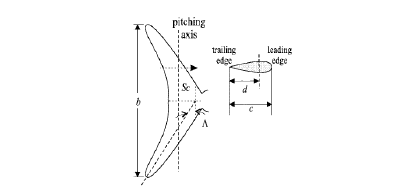
\includegraphics[scale=0.75]{caudalfinview.png}
    \caption{Lateral view of caudal fin. Adapted from \cite{magnuson}}
    \label{fig:caudalfinview}
\end{figure}
Fish swims by exerting force against the surrounding water. The main forces acting on fish during swimming are the fish's weight, buoyancy, and hydrodynamic lift in vertical direction, and thrust and drag in horizontal direction \citep{magnuson}, illustrated in figure \ref{fig:force}. Laterally, the forces cancel out while in horizontal direction, there exist a net force backwards, which propels the fish forward according to Newton's third law on motion.\par
\begin{figure}[H]
    \centering
    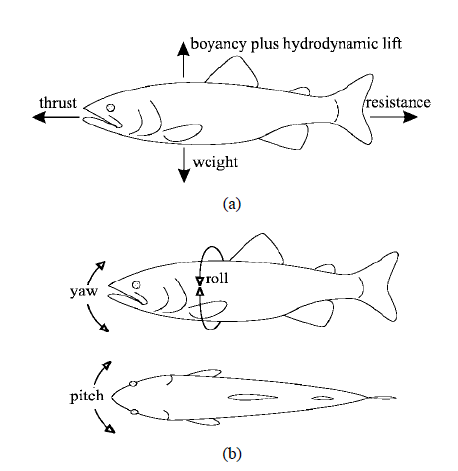
\includegraphics[scale=0.5]{force.png}
    \caption{Forces acting on a swimming fish (a). Dynamics variable definitions (b). Adapted from \citet{magnuson}}
    \label{fig:force}
\end{figure}
Investigation of fish hydrodynamics has led to several findings \citet{lauder1}. It is outlined that fish has several key characteristics in it's locomotion. Fish is statically unstable, which leads to the need of constant active control of fin, even during hovering. Fish fin is also flexible, which enables fish to direct the force generated by the fins and plays a role in thrust generation. This flexibility along with the existence of fin rays make it possible for fish to change it's fin curvature, enabling the fish to resist more hydrodynamic load. It is also observed that fish fins move in a complex three-dimensional manner. Experimental setup usually treated fish fin as undulating model, however the observation that three-dimensional motion is present even in steady locomotion of fish make this treatment inadequate in understanding fish fin function. This three-dimensionality effect leads to the understanding that dorsal and anal fin also contributes as much thrust as the tail. This also leads to the speculation that difference in locomotion patterns of fish is the result of different three-dimensional effect and fin use. However, if fish from different species with different swimming characteristics is observed in it's horizontal section during swimming, it is found that fish swims in similar manner accross species, which leads to the conclusion that 2D patterns of undulation is very similar among fishes.\par
While fish fin motion might seem complex at a glance, usually caudal fin oscillating motion is simplified into pitching and heaving motion only. Figure \ref{fig:caudalfinkinem} illustrate a fish during it's motion.
\begin{figure}[H]
    \centering
    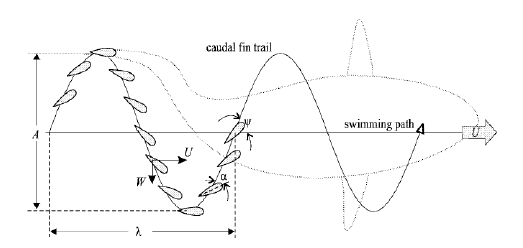
\includegraphics[scale=0.75]{caudalfinkinem.png}
    \caption{Lateral view of caudal fin. Adapted from \citet{magnuson}}
    \label{fig:caudalfinkinem}
\end{figure}
Amplitude $A$ is the maximum width of heaving motion of the fin, wavelength $\lambda$ refers to the length of wave that the fish body mimics as it swims, angle of attack $\alpha$ refers to the angle of the chord line with respect to the caudal fin's trail, feather angle $\Psi$ is the angle between the fin trail and it's swimming path, $U$ and $W$ refers to the swimming velocity parallel and perpendicular to the fish's swimming path, respectively \citep{sfakiotakis}.
\subsection{Derivation of the Flow Equation}
\label{sec:8}
Consider a 3-D flapping body immersed in an incompressible Newtonian fluid. Following \citet{borazjani}, the Navier-Stokes equation that has been non-dimensionalised by characteristic reference velocity $U$ and fin length $L$ can be rewritten as:
\begin{equation}
    \nabla^{*} \cdot \mathbf{u}^{*} = 0
    \label{eq:consofmass}
\end{equation}
\begin{equation}
    \frac{\partial \mathbf{u}^{*}}{\partial t^{*}} + \left(\mathbf{u}^{*} \cdot \nabla^{*} \right) \mathbf{u}^{*} = -\nabla^{*}p^{*} + \frac{1}{Re} \nabla^{*^{2}}\mathbf{u}^{*}
    \label{eq:consofmomentum}
\end{equation}
Equation \ref{eq:consofmass} describe the conservation of mass during the fluid motion, which states that the volume of the fluid element does not change during motion. The right hand terms of equation \ref{eq:consofmomentum}, which is basically the Newton's second law on motion or conservation of momentum, describes the effect of pressure and viscosity on the motion of a fluid. Reynolds number, denoted by $Re$ describes the ratio between inertial effect and viscous dissipation. It can then be inferred that, depending on the swimming condition, as $Re$ becomes higher, the viscous effect of the fluid can be neglected, and vice versa.\par
Rewriting equation \ref{eq:consofmomentum} in terms of vorticity can be more helpful as pressure distribution is more difficult to measure experimentally \citep{dea}. Non-dimensionalised vorticity $\boldsymbol{\omega}^{*}$ is defined as:
\begin{equation}
    \boldsymbol{\omega}^{*} = \nabla^{*} \times \mathbf{u}^{*}
    \label{eq:defineomega}
\end{equation}
Taking the curl of equation \ref{eq:defineomega} and plugging in definition from \ref{eq:consofmomentum} will yield:
\begin{equation}
    \frac{\partial \boldsymbol{\omega}^{*}}{\partial t^{*}} = \nabla^{*} \times \left(\mathbf{u}^{*} \times \boldsymbol{\omega}^{*} \right) + \frac{1}{Re} \nabla^{*^{2}} \boldsymbol{\omega}^{*}
    \label{eq:consofvorticity}
\end{equation}
Equation \ref{eq:consofvorticity} is the same as equation \ref{eq:consofmomentum}, written in terms of non-dimensionalised vorticity $\boldsymbol{\omega}^{*}$.\par
To derive an expression for force generated by a fish fin in mathematical form, thin airfoil theory will be used. Integrate small vorticity element over the surface area $S$ of an airfoil, bounded by closed contour $\Sigma$:
\begin{equation}
    \oint\limits_{\Sigma} \mathbf{u}^{*} \cdot\, \mathrm{d}l^{*} = \iint\limits_{S} \boldsymbol{\omega}^{*} \cdot \mathbf{n}^{*}\, \mathrm{d}S^{*}
    \label{eq:vortintegrate}
\end{equation}
to obtain circulation $\Gamma$. Applying Kutta-Jokowski theorem and adding the circulation term, force can be written in mathematical form as:
\begin{equation}
    \mathbf{F} = -\rho\frac{\mathrm{d}}{\mathrm{d}t} \int\limits_{R} \mathbf{r} \times \boldsymbol{\omega}\, \mathrm{d}R+ \rho\frac{\mathrm{d}}{\mathrm{d}t} \int\limits_{S} \mathbf{v} \cdot \mathbf{n}\, \mathrm{d}A
    \label{eq:forcevort}
\end{equation}
$\mathbf{v}$ is defined as induced velocity, which exist due to the presence of non-zero vorticity $\boldsymbol{\omega}$ of a small fluid element $\mathrm{d}V$ at a distance $\mathbf{r}$ from the region of interest. According to Biot-Savart law, the induced velocity can be expressed as:
\begin{equation}
    \mathbf{v} = \frac{1}{4\pi} \int\limits_{V} \boldsymbol{\omega} \times \frac{\mathbf{r}}{\mathbf{r}^{3}}\, \mathrm{d}V
    \label{eq:biotsavartvelo}
\end{equation}
Equation \ref{eq:forcevort} states that the force acting on an airfoil is generated by the vorticity arisen from the movement of the airfoil, expressed in the first term on the right hand side of the equation and inertial force of the fluid displaced by the airfoil body, shown in the second term of the right hand side of the equation.
\subsection{Scaling Parameters}
\label{sec:9}
The introduction of scaling parameters, combination of multiple parameters into a set of non-dimensional parameters, helps reduce the number and complexity of parameters involved in the experiment \citep{shyy}. There are three common scaling parameters used in caudal fin analysis:
\begin{enumerate}
    \item Reynolds number $Re$: the ratio between fluid inertia and viscous dissipation.
    \begin{equation}
        Re = \frac{U L}{\nu}
    \end{equation}
    where $U$ denotes freestream velocity of the fluid, $L$ signifies reference length, and $\nu$ denotes kinematic viscosity. For scaled objects with identical $Re$, the value of non-dimensional fluid properties and force is the same.
    \item Strouhal number $St$: the ratio of fin flapping frequency to forward swimming speed.
    \begin{equation}
        St = \frac{f A}{U}
    \end{equation}
    where $f$ denotes the flapping frequency, $A$ signifies the width of the wake in lateral direction, and $U$ denotes freestream velocity of the fluid.
    \item Reduced frequency $k$: a scaling parameters similar to Strouhal number, but represents flow unsteadiness better than Strouhal number.
    \begin{equation}
        k = \frac{\pi f L}{U}
    \end{equation}
    where $f$ denotes the flapping frequency, $L$ signifies the length of the fin, and $U$ denotes freestream velocity of the fluid.
\end{enumerate}
\subsection{Hydrodynamics of Caudal Fin}
\label{sec:10}
Thrust generated by undulatory motion is similar to that of thrust generated by propeller, by producing localised thrust wake with an observable momentum jet, as illustrated in figure \ref{fig:vortex}.
\begin{figure}[H]
    \centering
    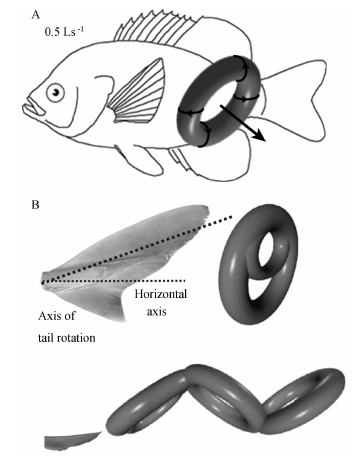
\includegraphics[scale=0.5]{vortex.png}
    \caption{Vortex ring around bluegill sunfish (A) and the tail of leopard sharks (B). Adapted from \cite{lauder1}}
    \label{fig:vortex}
\end{figure}
In the case of fish, thrust is generated by a backward-moving propulsive wave that extends to it's caudal fin \citep{sfakiotakis}. A foil (or in this case, a fin) in steady forward motion combined with steady-state harmonic heaving and pitching motion produces thrust through the formation of a flow downstream from the trailing edge, which when averaged over a period of oscillation has the form of a jet \citep{anderson}. This undulatory motion also generated a large side force that is speculated to be necessary for maintaining stability or simply a consequence of the undulatory motion itself \citep{lauder1}.\par
Particle image velocimetry (PIV) method has shed some light on the behaviour of water around a flapping fin in the recent years by allowing visualisation of water flow around the body of swimming fish. In this method, laser light is focused into a 2D light sheet and images are then obtained from high-speed videos of particles moving with the flow, which gives detailed time-dependent description of water flow patterns, calculation of wake vorticity and estimation of force. This 2D PIV approach has been extended into volumetric 3D imaging capability, which provides instantaneous 3D flow reconstructions of the wake produced by the fish' body and fins during swimming \citep{lauder2}.\par
Caudal fin produced wake consisted of a series of string counter-rotating vortices, typical of structure of a series of linked in vortex rings as shown in figures \ref{fig:wake1} and \ref{fig:wake2}. Between each pair of counter-rotating vortices, a jet of high velocity of flow was formed \citep{nauen}.\par
\begin{figure}[H]
    \centering
    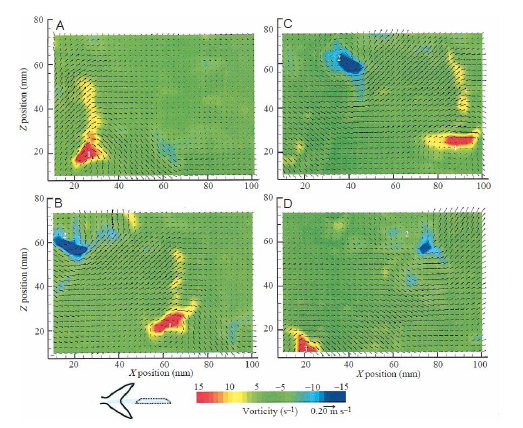
\includegraphics[scale=0.75]{wakepiv1.png}
    \caption{The time course of vortex production over approximately one tail beat of a Scomber japonicus 24 cm in fork length (FL) swimming at 1.2 FL s–1. The distal tips of the caudal fin were positioned approximately 1 cm to the left of the flow fields shown. The caudal fin was moving through the horizontal (XZ) light sheet at the position of the fin’s lateral. Flow velocity is represented by the black vectors plotted over a color background indicating flow vorticity. Vortices in the wake are numbered consecutively in the order in which they are shed from the caudal fin. Adapted from \citet{nauen}}
    \label{fig:wake1}
\end{figure}
\begin{figure}[H]
    \centering
    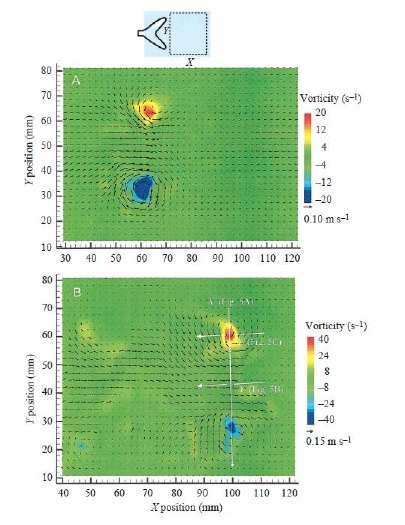
\includegraphics[scale=0.75]{wakepiv2.png}
    \caption{Views if the wake in the vertical (XY) plane of an individual of Scomber japonicus 26 cm in fork length swimming steadily at speeds of 1.2 \textit{FL s}\textsuperscript{-1} (A) and 2.2 \textit{FL s}\textsuperscript{-1}, where \textit{FL} is the fork length (B). Flow velocity is represented by black vectirs plotted over a color background indicating vorticity. At both swimming speeds, the caudal fin sheds one pair of counter-rotating vortices with central jet of high velocity per stroke.}
    \label{fig:wake2}
\end{figure}
\begin{figure}[H]
    \centering
    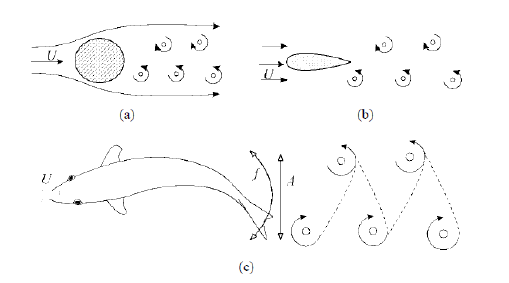
\includegraphics[scale=0.75]{karmanstreet.png}
    \caption{The Karman street generates a drag force for either (a) bluff or (b) streamlined bodies, placed in a free stream. (c) The wake of swimming fish has reverse rotational direction, associated with thrust generation.}
    \label{fig:karmanstreet}
\end{figure}
As caudal fin moves back and forth, the wake left behind the tail of undulatory swimmer is a staggered array of trailing discrete vortices of alternating sign as shown in figure \ref{fig:karmanstreet}. This reversed rotational direction produced thrust instead of drag that is produced by the well-documented Karman vortex sheet. This propulsive wave traverse the fish body in opposite direction to the fish' overall movement and faster that the overall swimming speed \citep{sfakiotakis}.
\section{Fundamentals of Global Surrogate Assisted Genetic Algorithm}
\label{sec:11}
This subsection will explain the fundamentals of genetic algorithm used for optimisation process. The fundamentals of single objective genetic algorithm will be explained in \ref{sec:12}, the concept of surrogate modeling and it's construction with Kriging method will be explained in \ref{sec:13}, and the coupling between GA and surrogate modeling will be outlined in \ref{sec:14}.
\subsection{Fundamentals of Single-Objective Genetic Algorithm}
\label{sec:12}
Optimisation is defined as the process of adjusting a set of input variables to a mathematical process or function i.e fitness function in order to find maximum or minimum output or result i.e fitness \citep{haupt}. There are many approaches to optimise a function, among them are analytical optimisation and natural optimisation. Analytical optimisation is based on the idea that the optimum of a function is reached when the first derivative of a function is equal to zero. This begs the question: what if the function is not explicit? Or continuous? What if the fitness is a function of many variables? Realising that many cases in real-life cannot be modeled in a straightforward manner renders analytical optimisation impractical. Natural optimisation approach is different from analytical approach in a sense that instead of finding the fitness function to obtain fitness, natural optimisation moves intelligently from point to point in a predefined search space to obtain fitness, or in simple terms ``intelligent trial-and-error''. One such approach is called genetic algorithm (GA) which is based on principle of genetics and natural selection.\par
In GA, a set of variables is treated as a population composed of single individuals which is allowed to evolve according to the principles of genetic recombination and natural selection under  a set of selection rules to obtain fitness value. GA was first developed by John Holland and David Goldberg in the 70s to solve gas-pipeline transmission control problem. GA is further divided based on the amount of objectives into single-objective where the fitness of a single fitness function and multi-objective where one evaluates the fitness(es) of several fitness functions from similar input. How the input of a variable is formulated also differs GA: binary GA, where the input is represented as a string of encoded binary numbers, which is simple and similar to how chromosomes work in nature but also unsuitable for continous, multi-variable or high-precision problems; and real GA (RGA) where each individual is represented with floating-point numbers \citep{haupt}.\par
\begin{figure}[H]
    \centering
    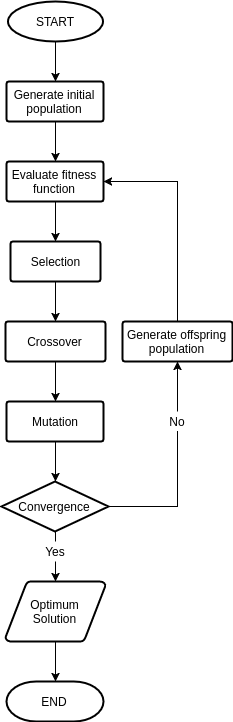
\includegraphics[scale=0.7]{flowchartrga.png}
    \caption{Flowchart of basic real single-objective genetic algorithm.}
    \label{fig:flowchartrga}
\end{figure}
Flowchart shown in figure \ref{fig:flowchartrga} shows that the process of RGA to find the fitness value of fitness function $f(\mathbf{x})$ with input $\mathbf{x} = [\mathbf{x}^{(1)}, \mathbf{x}^{(2)}, \ldots, \mathbf{x}^{(N)}]^{T}$ can be divided into five steps which consists of:
\begin{enumerate}
    \item Initial population generation

    GA begins with generating random $N_{pop} \times N_{var}$, where $N_{var}$ is the number of variables and $N_{pop}$ is the number of individuals inside the population on each generation. All variables are normalised into real numbers $x_{norm}$ between $[0, 1]$ convenience sake. Unnormalised variable $x$ is obtained from the following equation:
    \begin{equation}
        x = x_{l} + \left(x_{h} - x_{l}\right)x_{norm}
        \label{eq:norm2unnorm}
    \end{equation}
    where $x_{l}$ and $x_{h}$ are the lowest and highest number in the variable range, respectively.
    \item Fitness function evaluation

    Individuals are then evaluated using a known fitness function $f(\mathbf{x})$. If $f(\mathbf{x})$ is unknown, then each individual in the population is evaluated through either numerical simulation or experiment.
    \item Selection

    Population are selected in a similar way to Darwinian natural selection to form a mating pool. There are several methods to perform selection such as top-to-bottom, random, weighted, cost and tournament pairing. Tournament selection method is used for selection method in this thesis. In this approach, two individuals are randomly selected from the population and undergoes mating competition where the individual with lower fitness wins (i.e enter the mating pool). This process will produce a $N_{pop} \times N_{var}$ mating pool matrix for crossover process \citep{haupt}.
    \item Crossover

    Crossover is the analogy to reproduction in real-life evolution process where two individuals ``marry off'' to create a new individual i.e an offspring. The method for crossover used in this thesis is simulated binary crossover (SBX). SBX is an adaptive search method where the crossover probability of distribution depends on how close an offspring is to it's parents. As the solution converges, the offspring becomes more similar to it's parents \citep{deb}.
    \item Mutation

    Just like it's natural counterpart, mutation in GA is an alteration introduced to the offsprings that occurs constantly according to a small mutation probability. In GA process, mutation prevents the solution from converging too quickly at a local optimum.
\end{enumerate}
\subsection{Global Surrogate-Assisted Genetic Algorithm (G-SAGA)}
\label{sec:13}
From \ref{sec:12} it is implied that the larger the population, the more robust the optimisation. Consider now a population consisting of 100 individuals and GA iteration that loops until 100 generation. This means that one have to do 10000 experimental or numerical runs, which is expensive. To overcome this problem, a surrogate model was used in this thesis. Surrogate models are models that are built to approximate the ``true'' fitness function $f(\mathbf{x})$ to decrease computational or experimental cost massively. It also provides insight on how an input $\mathbf{x}$ affects the output $\mathbf{y}$ (\cite{ong}). If a case is represented mathematically as:
\begin{equation}
    y = f(\mathbf{x})
    \label{eq:truefcn}
\end{equation}
then the surrogate model is an approximation of the form
\begin{equation}
    \hat{y} = \hat{f}(\mathbf{x})
    \label{eq:approxfcn}
\end{equation}
such that
\begin{equation}
    y = \hat{y} + \epsilon
    \label{eq:true2approx}
\end{equation}
It can then be inferred that, in a sense, surrogate modeling process is a surface fitting process that mimics the real behaviour of a physical process. In this thesis, Kriging was chosen to be the surrogate modeling method.\par
\begin{figure}[H]
    \centering
    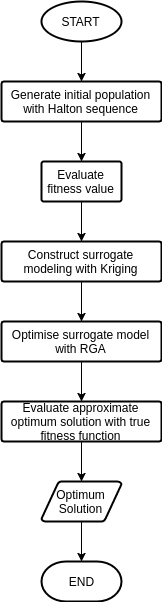
\includegraphics[scale=0.7]{flowchartkrig.png}
    \caption{Flowchart of surrogate-assisted genetic algorithm.}
    \label{fig:flowchartkrig}
\end{figure}
Figure \ref{fig:flowchartkrig} illustrated the flowchart of surrogate-assisted genetic algorithm. As with basic GA, G-SAGA begins with population generation $N_{pop}$. This population was generated using a sampling plan algorithm called Halton sequence \citep{bimo}. Each individuals of $N$ amount are then evaluated through experiment to obtain responses $\mathbf{y} = [y^{(1)}, y^{(2)}, \ldots, y^{(N)}]^{T}$ that correlates to sample set $\mathbf{x} = [\mathbf{x}^{(1)}, \mathbf{x}^{(2)}, \ldots, \mathbf{x}^{(N)}]^{T}$. The evaluation result is then fitted using Kriging to obtain the surrogate model $\hat{f}(\mathbf{x})$ that approximate the true fitness function $f(\mathbf{x})$. Approximate optimum solution $\mathbf{x}_{opt}$ was obtained by optimising the surrogate model $\hat{f}(\mathbf{x})$ using RGA. This approximate optimum solution $\mathbf{x}_{opt}$ is finally evaluated using experiment to generate the best fitness value $y_{opt} = f(\mathbf{x}_{opt})$. Using this approach, instead of having to do 10000 times experimental runs to obtain an optimum solution, one only have to do 100 experimental runs to obtain the initial correlation between $y$ and $\mathbf{x}$ and run one more experiment on the optimum solution $\mathbf{x}_{opt}$, reducing the workload up to 99\%. This thesis used G-SAGA code created by \citet{bimo} for single objective case with few modifications to connect the algorithm to the experimental system.
\subsection{Fundamentals of Kriging}
\label{sec:14}
Kriging is defined as design and analysis of computer experiments model \citep{sacks} or Gaussian process regression \citep{williams}. One may think of it as a n-dimensional curve or surface fitting method.\par
Given a set of $n$ noise-free sample data, $\mathbf{x} = [\mathbf{x}^{(1)}, \mathbf{x}^{(2)}, \ldots, \mathbf{x}^{(n)}]^{T}$ that correlates to response $\mathbf{y} = [y^{(1)}, y^{(2)}, \ldots, y^{(n)}]^{T}$. The relation between sample set and responses is denoted using a set of vectors
\begin{equation}
    \mathbf{Y} =
        \begin{bmatrix}
            Y(\mathbf{x}^{(1)}) \\
            Y(\mathbf{x}^{(2)}) \\
            \vdots \\
            Y(\mathbf{x}^{(n)})
        \end{bmatrix}
    \label{eq:set2resp}
\end{equation}
Each elements in vector $\mathbf{Y}$ are connected with each other with a basis function
\begin{equation}
    \mathrm{cor}[Y(\mathbf{x}^{(i)}),Y(\mathbf{x}^{(l)})] = \exp\left(-\sum_{j=1}^{k}\boldsymbol{\theta}_{j}\lvert x_{j}^{(i)} - x_{j}^{(l)}\rvert^{\mathbf{p}_{j}}\right)
    \label{eq:basisfcn2cor}
\end{equation}
\par
The right hand side term of equation \ref{eq:basisfcn2cor} is a basis function for a surrogate model construction called Kriging. In kriging, the basis function $\psi$ is expressed as:
\begin{equation}
    \psi^{(t)} = \exp\left(-\sum_{j=1}^{k}\boldsymbol{\theta}_{j}\lvert x_{j}^{(i)} - x_{j}^{(l)}\rvert^{\mathbf{p}_{j}}\right)
    \label{eq:basiskriging}
\end{equation}
Equation \ref{eq:basiskriging} basically gives the basis needed to construct the Kriging model by solving for $\boldsymbol{\theta}$ and $\mathbf{p}_{j}$, where $\boldsymbol{\theta} = [\theta_{1}, \theta_{2}, \dots, \theta_{k}]^{T}$ is the basis vector (similar to $\hat{i}$, $\hat{j}$, and $\hat{k}$ in Cartesian basis) and $\mathbf{p}_{j} = [p_{1}, p_{2}, \dots, p_{k}]^{T},\, \mathbf{p}_{j}\in[1,2]$ is the exponent vector.\par
The construction of surrogate model with Kriging starts with maximisation of likelihood function $L$, expressed in natural logarithmic $\ln$ as
\begin{equation}
    \ln L = -\left(\frac{n}{2}\ln(2\pi) + \frac{n}{2}\ln(\sigma^{2}) + \frac{1}{2}\ln\lvert\boldsymbol{\Psi}\rvert + \frac{\left(\mathbf{y} - \mathbf{1}\mu\right)\boldsymbol{\Psi}^{-1}\left(\mathbf{y} - \mathbf{1}\mu\right)}{\sigma^{2}}\right)
    \label{eq:likelihoodfcn}
\end{equation}
where $\sigma^{2}$ is the variance, $\mathbf{1}\mu$ is the mean of random vector $\mathbf{Y}$, and $\mathbf{1}$ is an $1 \times n$ column vector consisting of ones. $\boldsymbol{\Psi}$ is Gram matrix defined as
\begin{equation}
    \boldsymbol{\Psi} =
        \begin{bmatrix}
            \mathrm{cor}[Y(\mathbf{x}^{(1)}),Y(\mathbf{x}^{(l)})] & \dots & \mathrm{cor}[Y(\mathbf{x}^{(1)}),Y(\mathbf{x}^{(n)})] \\
            \vdots & \ddots & \vdots \\
            \mathrm{cor}[Y(\mathbf{x}^{(n)}),Y(\mathbf{x}^{(l)})] & \dots & \mathrm{cor}[Y(\mathbf{x}^{(n)}),Y(\mathbf{x}^{(n)})]
        \end{bmatrix}
    \label{eq:grammat}
\end{equation}
by deriving equation \ref{eq:likelihoodfcn} once and equating it with zero, maximum likelihood estimates (MLEs) for variables $\sigma^{2}$ and $\mu$ is obtained
\begin{equation} \label{eq:sigmamu}
\begin{split}
    \hat{\mu} &= \frac{\mathbf{1}^{T}\boldsymbol{\Psi}^{-1}\mathbf{y}}{\mathbf{1}^{T}\boldsymbol{\Psi}^{-1}\mathbf{1}} \\
    \hat{\sigma}^{2} &= \frac{\left(\mathbf{y} - \mathbf{1}\mu\right)^{T}\boldsymbol{\Psi}^{-1}\left(\mathbf{y} - \mathbf{1}\mu\right)}{n}
\end{split}
\end{equation}
substituting equation \ref{eq:sigmamu} to \ref{eq:likelihoodfcn} and removing constant terms from the same equation, a simplified function called the ``concentration $\ln$-likelihood function'' is obtained
\begin{equation}
    \ln(L) \approx -\left(\frac{n}{2}\ln(\sigma^{2}) + \frac{1}{2}\lvert\boldsymbol{\Psi}\rvert\right)
    \label{eq:conclikelihood}
\end{equation}
following \citet{forrester}, by deriving likelihood function $L$, the surrogate model $\hat{f}(\mathbf{x})$ of a fitness function $f(\mathbf{x})$ is
\begin{equation}
    \hat{f}(\mathbf{x}) = \hat{\mu} + \boldsymbol{\psi}^{T}\boldsymbol{\Psi}^{-1}\left(\mathbf{y} - \mathbf{1}\hat{\mu}\right)
    \label{eq:surrogatefcn}
\end{equation}
where $\boldsymbol{\psi} = [\psi^{(1)}, \psi^{(2)}, \dots, \psi^{(n)}]^{T}$ is the basis function vector. Equation \ref{eq:surrogatefcn} shows that surrogate model $\hat{f}(\mathbf{x})$ is a function of basis vector $\boldsymbol{\theta}$ and exponent vector $\mathbf{p}_{j}$ inside $\boldsymbol{\psi}$ and $\boldsymbol{\Psi}$. This method is called Kriging interpolation.\par
Recall that Kriging interpolation that is derived previously assumes that the sample set is noise-free. However, there exist random noise during force measurement in towing tank experiment during fitness evaluation. To filter noisy sample data, a regression constant $\lambda$ is introduced into equation \ref{eq:surrogatefcn} so that it becomes
\begin{equation}
    \hat{f}(\mathbf{x}) = \hat{\mu}_{r} + \boldsymbol{\psi}^{T}\left(\boldsymbol{\Psi} + \lambda\mathbf{I}\right)^{-1}\left(\mathbf{y} - \mathbf{1}\hat{\mu}_{r}\right)
    \label{eq:surrogatefcnmod}
\end{equation}
where
\begin{equation}
    \hat{\mu}_{r} = \frac{\mathbf{1}^{T}(\boldsymbol{\Psi} + \lambda\mathbf{I})^{-1}\mathbf{y}}{\mathbf{1}^{T}(\boldsymbol{\Psi} + \lambda\mathbf{I})^{-1}\mathbf{1}}
    \label{eq:mur}
\end{equation}
\par
In this thesis, the exponent vector was set to a constant value $\mathbf{p}_{j} = 2$, while the basis vector $\boldsymbol{\theta}$ was set in the range $\boldsymbol{\theta}\in[10^{-3},10^{2}]$. The value of regression constant $\lambda$ was set in the range $\lambda\in[10^{-6},1]$.\par

% Detail of your thesis. This should be where you describe your work e.g code setup, experimental setup, design process, etc. Write it in chapters/bab3.tex
\chapter{Experimental System Design and Setup}
As the title suggest, this chapter describes the design process and the resulting experimental system setup. Section \ref{sec:setup} describes the general overview of the experimental setup: subsystems that builds the whole experimental system, the ``job description'' of each subsystems, and how each subsytems relate to each other to run the whole experimental system. Sections \ref{sec:trans}, and \ref{sec:measure} describes in detail the components, how each components work, and how those components relate to each other to build translational, rotational, force measuring, respectively. The last section (Sec. \ref{sec:specimenmodel}) describes the specimen that was used in this thesis, including design consideration, production process and it's mechanical properties.\par
\section{Experimental Setup in General}
\label{sec:setup}
The experiment was conducted in towing tank facility in Aerogasdynamics Laboratory in Aerospace Engineering programme, Faculty of Mechanical and Aerospace Engineering, Bandung Institute of Technology. The towing tank is glass-walled and 200 $\times$ 60 $\times$ 60 cm in length, width, and height, respectively. The towing tank was filled with typical water (density $\rho$ = 1000 kg/m$^{3}$ and kinematic viscosity $\nu$ = 1 $\times$ 10$^{-6}$ m/s$^{2}$) up to 43 cm in height. A carbon fiber carriage was attached to two shafts with four linear bearings above towing tank to carry a specimen, a servo for rotational motion, and a load cell for force measurement. The carriage was connected via belt-and-pulley mechanism to a stepper motor for translational motion.\par
The experimental system can be divided into three major subsystems: traversing system for moving the specimen along translational (i.e forward and backward) plane, force measurement system for measuring the instantaneous force acting on the specimen. Figure \ref{fig:schemeexpforce} describes the relationship between each subsystems to build the experimental setup for force measuring purpose. These subsytems will be explained in detail in the following sections.
\begin{figure}[H]
    \centering
    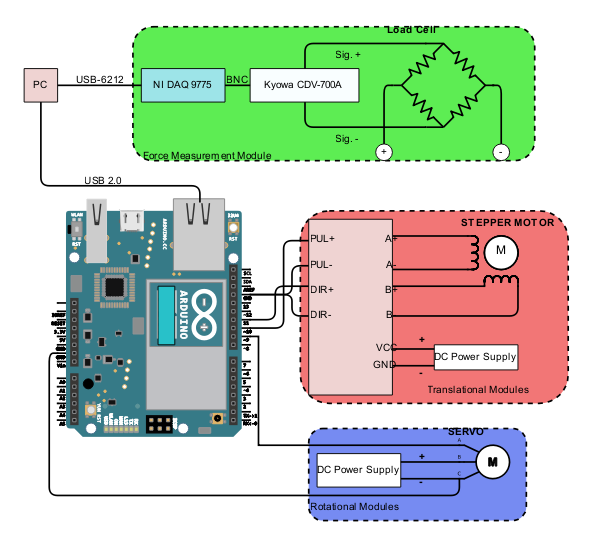
\includegraphics[scale=0.75]{schemeexpforce.png}
    \caption{Subsystem schematic for force measurement experimental runs.}
    \label{fig:schemeexpforce}
\end{figure}
It is also worth noting that it is desirable to have an automated experimental system, which means that all system must be connected to a personal computer and controlled by a software. In this case, the hardware controller used was an Arduino Uno R3 board. Arduino is a microcontroller board based on ATmega328, an AVR 8-bit processor, esentially a mini computer suitable for repeating tasks. Arduino Uno has 14 digital I/O pins, 6 of which can be used as PWM outputs, and 6 analog input pins. The softwares are Arduino package for traversing system and MATLAB R2015a for data and image acquisition and also optimisation algorithm. In traversing system, Arduino Uno R3 board was used to connect stepper motor and servo motor to a personal computer and a code was built to control both motors. A code based on Arduino language (which in turn is based on C++) was made as an interface between user, computer, and hardwares related to traversing purpose and a code in MATLAB was built as an interface for data acquisition and optimisation needs. Both of those softwares communicate through serial communication native to Arduino and MATLAB. The towing tank facility can be seen in figures \ref{fig:setupirl} and \ref{fig:setupdatairl}.
\begin{figure}[H]
    \centering
    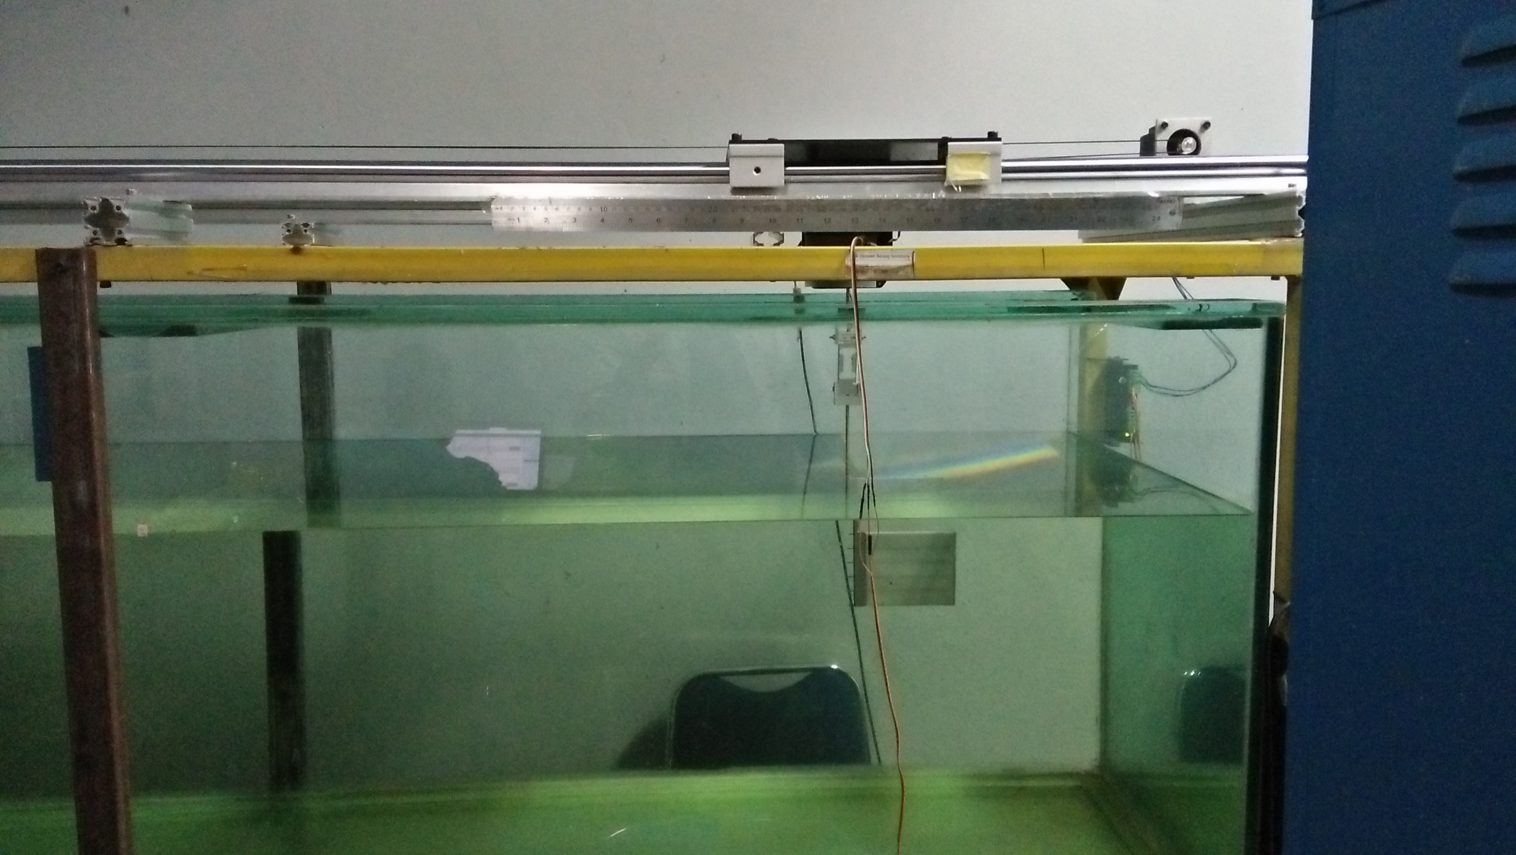
\includegraphics[scale=0.6]{setupirl.png}
    \caption{Towing tank experimental facility.}
    \label{fig:setupirl}
\end{figure}
\begin{figure}[H]
    \centering
    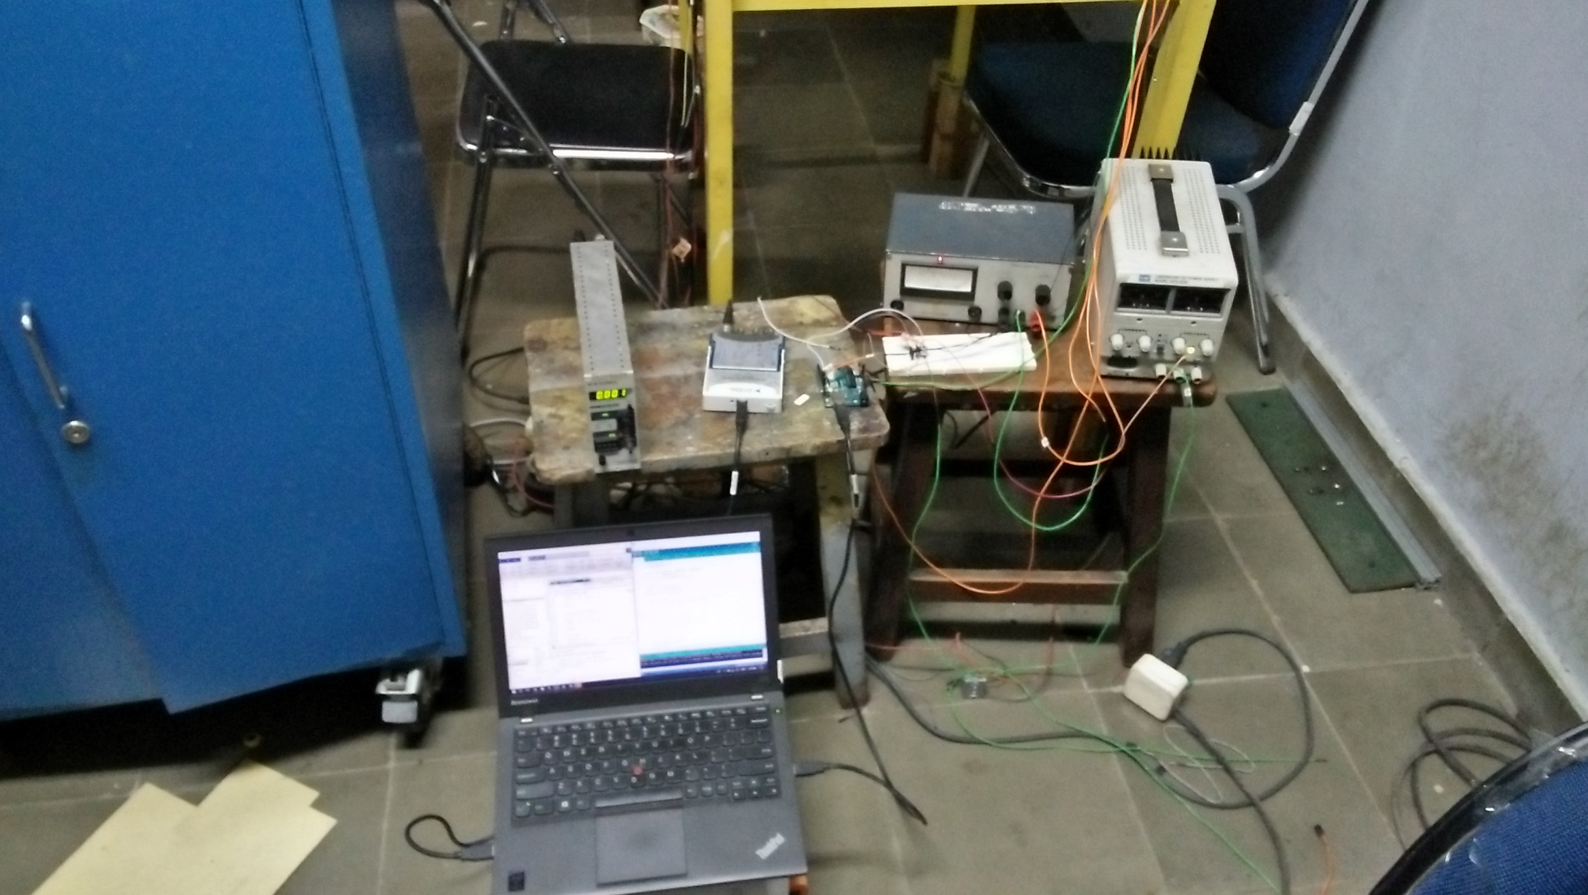
\includegraphics[scale=0.6]{setupdatairl.png}
    \caption{Towing tank experimental control panel.}
    \label{fig:setupdatairl}
\end{figure}
\section{Traversing System}
\label{sec:trans}
Traversing system dictates how does the specimen moves forward, backward, and rotates during the duration of experiment. This system is further divided into two smaller systems: translational system, described in subsection \ref{sec:forback}, which deals with how does a specimen moves forward and backward, and rotational system, described in subsection \ref{sec:rotate} which deals with how does a specimen moves rotationally.
\subsection{Translational System}
\label{sec:forback}
Translational system is indicated with red background on figures \ref{fig:schemeexpforce} and \ref{fig:schemeexpimage}. The system consists of one stepper motor, one stepper motor driver, and one DC power supply. The system was designed to move the carbon fiber carriage backward and forward on a straight line. To do that, the carbon fiber carriage was mounted on four 20 mm linear bearings which in turn rest on two 20 mm circular shafts. The carbon fiber carriage was also connected to two pulleys on both ends of the water tank via a 2 mm pitch rubber belt. On one end, a timing pulley with matching pitch was mounted on stepper motor shaft and on the other end a pitchless idler pulley was mounted on a custom aluminium frame. The correlation between motor rotational speed in rps (rotation per second) denoted by $\omega$ and resolution of microstep (i.e how many pulses are generated for one motor shaft revolution) denoted by $n$ is:
\begin{equation}
    \omega = \frac{f}{n}
    \label{eq:pprtorotspeed}
\end{equation}
where $f$ is the input pulse frequency. For this experiment, the resolution of microstep was set at 1600 pulse/rev and the driver is rated at maximum 200 kHz pulse frequency. Therefore, the translational speed of the carriage can be written as:
\begin{equation}
    v = \pi\omega d
    \label{eq:omega2vel}
\end{equation}
where $d$ is the diameter of the motor shaft, $d$ = 6.35 mm. It should be noted that controlling the velocity and distance traveled by the carriage, manually adjusting the pulse input or microstep resolution is not required. A more convenient method is to use a native Arduino library to control direction, distance, and velocity \texttt{\textcolor{blue}{<AccelStepper.h>}}.\par
A Leadshine NEMA23 2-phase stepper motor was connected to Leadshine DM542 stepper motor driver pins following the available manual written in the stepper motor. The stepper motor was powered using a DC power supply connected to V+ and GND pin for positive voltage and negative voltage, respectively. The power supply was able to supply 0 - 50 V DC and the stepper motor driver itself requires minimum 20 V DC to operate. The rest of the pins was connected to digital input pins on an Arduino R3 Uno board. PUL+ pin which generates the pulse or step needed to rotate the motor shaft was connected to digital pin number 10 on Arduino R3 Uno board, DIR+ pin which governs the direction of motor shaft rotation (i.e clockwise or counter-clockwise) was connected to digital pin number 11, PUL- and DIR- were connected to GND pin.\par
\subsection{Rotational System}
\label{sec:rotate}
To mimic oscillating motion of a fin, rotational system was designed to fulfill said purpose. This system can rotate fin panel by rotating the load cell which was placed above the fin panel supported by a circular bar. This motion was actuated using Futaba S3003 servo placed inside a box along with two roller bearings attached inside the box to keep the circular bar supporting the fin straight. Two connectors held the bar between servo motor and the circular bar which was attached to the fin panel. The servo was powered by a laboratory power supply providing 5V. The positive terminal in the power supply was connected to the positive cable of the servo, the negative terminal was connected to the grounding terminal of the servo and was branched with a breadboard to be connected to the power ground in the Arduino board. The signal pin in the servo was connected to digital pin number 9 in the Arduino. Depicted in figure \ref{fig:rotvisual}, servo could change angle $\theta$ from $0^{0} - 180^{0}$ measured from a vertical line perpendicular to the translation direction by responding to a pulse length modulation with short duration between 1 - 2 ms. The motion of the servo was controlled using \texttt{\textcolor{blue}{<Servo.h>}} library native to Arduino.
\begin{figure}[H]
    \centering
    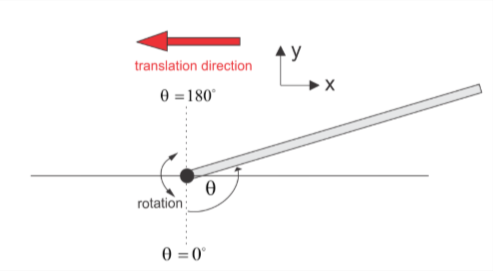
\includegraphics[scale=0.75]{rotvisual.png}
    \caption{Fin panel motion depiction.}
    \label{fig:rotvisual}
\end{figure}
\section{Force Measurement System}
\label{sec:measure}
An aluminium 300g single point load cell PW4MC3 (HBM) combined with Kyowa CDV-700A signal conditioner acted as two main component for force measuring. The load cell was used to measure the force acting on fin panel during it's motion and the signal conditioner acted as a signal amplifier and lowpass filter. Along with these two components, National Instruments DAQ board was used for data acquisition and this board was connected to a personal computer using USB-9215A which also acted as analog-to-digital converter which transmit sgnals from force measurement (an analog signal) to a personal computer (reads digital signal). The load cell has accuracy class C3 with OIML R60 test report and minimum sensitivity at 3 mN and the signal conditioner was operated in 2V bridge excitation voltage, RANGE in the value of 500 and 10 Hz cut-off frequency for analog lowpass filter.\par
As stated in section \ref{sec:rotate}, the load cell also rotates with fin panel, which means that the force data read by the load cell is force acting parallel to the chord line of the fin panel (denoted by $F_{load}$) in figure \ref{fig:freebodydiag}.
\begin{figure}[H]
    \centering
    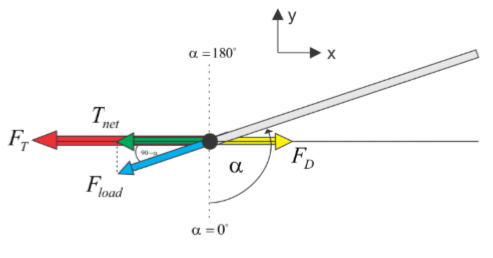
\includegraphics[scale=0.75]{freebodydiag.png}
    \caption{Free body diagram of forces acting on fin panel on xy-plane.}
    \label{fig:freebodydiag}
\end{figure}
Figure \ref{fig:freebodydiag} visualise forces acting along the translation direction experienced by the fin panel. The oscillating motion of the panel produce thrust force $F_{T}$ while drag force $F_{D}$ is the consequence of the panel translational motion. $F_{load}$ can be transformed into net thrust force $T_{net}$ by taking the x-direction component of $F_{load}$:
\begin{equation}
    T_{net} = F_{load} \cos \left(\alpha - 90\right) = F_{load} \sin\alpha
    \label{eq:load2net}
\end{equation}
The raw data obtained from load cell measurement was processed further to eliminate noise inherent to electrical systems. This was accomplished by imposing a digital lowpass filter to the raw data. The filter design was based on Butterworth n-th order filter with $f$ cutoff frequency, in this case, the filter order was chosen to be 4 and the cutoff frequency was specified at 2 Hz. The cutoff frequency value was determined from power spectrum density graph and the filter order was obtained based on previous thesis by \citet{hiroki}. The smoothing process was done using moving average method where the first element of each data was determined by taking the average of $n$ points forward. In the experiment, the points used to smooth the n-th data was determined at 100 points. This value was obtained through trial-and-error process.
\section{Variable-Stiffness Fin Model}
\label{sec:specimenmodel}
The fin model (Fig. \ref{fig:finpanel}) with varying stiffness was made using a 80 $\times$ 100 mm silicone rubber with six spring steel wires embedded within the silicon rubber during the production process. These spring steel wires acted as stiffeners and the stiffness of the whole specimen was varied by changing the length of the wire. This fin panel was glued to an aluminium board with matching thickness to prevent the fin panel from shearing, making sure that the flapping motion was strictly limited to flapping only. This board has six threaded holes on one of its surface that was used to prevent the wires from moving during flapping motion. The board was attached to the load cell with a 4 mm diametre circular bar and some part of the bar was lathed to fit the thickness of the fin (thickness = 3 mm) and to reduce the drag induced by the presence of the bar. The board and the bar was again glued to prevent the fin from slipping as slipping motion results in different amplitude output given a particular input.
\begin{figure}[H]
    \centering
    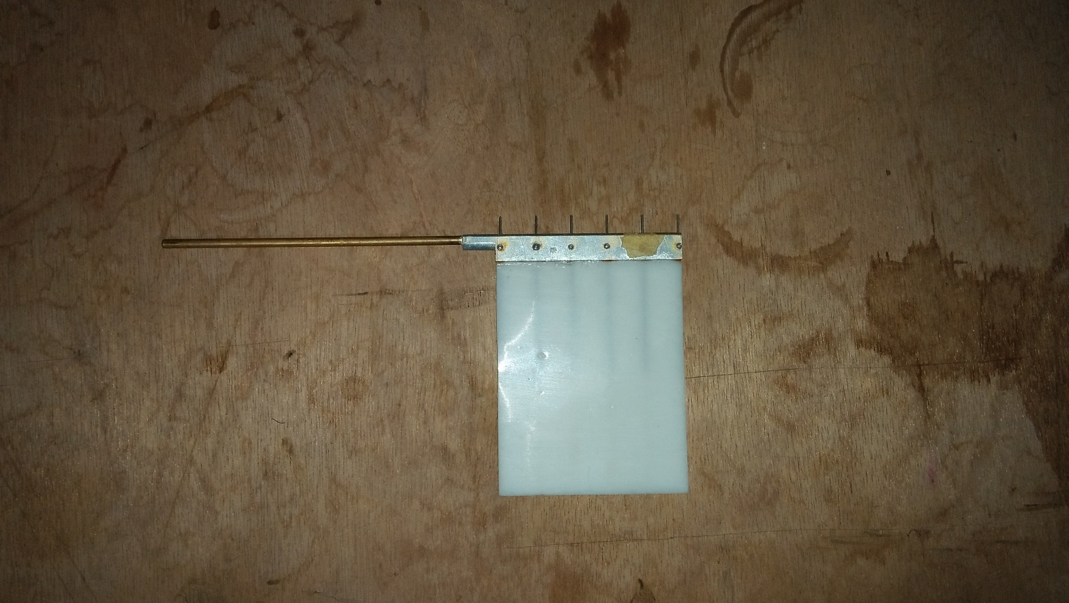
\includegraphics[scale=0.75]{specimen.png}
    \caption{The fin panel end product.}
    \label{fig:finpanel}
\end{figure}

The fin panel was made by pouring a 1:25 volumetric mixture of silicone rubber and catalyst ($E$ = 0.08 GPa) that had been vaccuumed in a pressurised vessel to a die made from acrylic boad matching the fin panel dimension. Within the die, six spring steel wires ($E$ = 207 GPa) was attached horizontally at it's ends that acts as the stiffener chord-wise and two wires was attached vertically at the leading and trailing edge to ensure stiffness along the thickness, thus ensuring that the panel does not twists as it flaps. The mixture inside the die was then vaccuumed again inside a pressurised vessel to ensure that there are no voids trapped inside the fin panel which may results in different material properties along the panel.\par
Changing the stiffness of the fin panel was simple: changing the spring wires length also changes the distribution of the material stiffness chord-wise, where the change of the material distribution also change the stiffness distribution which also leads to effective stiffness change of the whole panel. The wires was fastened using 1.27 mm set screws attached to six threaded holes in the aluminium board to keep the wires in place during motion. Changing the length was simply done by first loosening these set screws and pulling the wires using a pliers from the leading edge until the desired length and then refastened the set screws. To ensure the wires is already at the desired length, another wire was put inside the silicone from the trailing edge. This wire has a marking that indicates the previously desired wire length and if the wires barely touch each other, then the wire has reached the desired length.

% This should be where you put your result and your analysis. Write it in chapters/bab4.tex
\chapter{Results and Analysis}
In this chapter lies the most important piece of information: data and interpretation of said data. The first section (section \ref{sec:calib}) first outlined how to convert the data that the load cell actually records into the data that is relevant to this thesis. Section \ref{sec:optimiseresult} is the answer to the first objective of this thesis outlined in section \ref{sec:2}, which is what structural configuration yields the most optimum thrust. The next sections will seek to explain why and how the thrust is produced and the effect of flexibility to the generated thrust.\par
\section{Preliminary Calibration}
\label{sec:calib}
Before the experiment began, it should be made clear that the load cell used in this experiment does not directly generates force data. Instead, the load cell produce voltage as a result of strain change as a load is acting to the load cell, which in turn leads to the change of electrical resistance. Following the Wheatstone bridge circuit principle, this electrical resistance change leads to the change of voltage which can be translated into the load acting on the load cell.\par
To find the relationship between acting load and voltage output, a mini experiment to calibrate the load cell was conducted. The calibration was done by applying several predetermined loads ($W_{i}$) to the load cell and measuring the resulting voltage outputs ($V_{o}$) at a predetermined signal conditioner setup, which in this case the gain was set at 500$\times$, the lowpass frequency was set at 10 Hz and the sampling rate was set at 1000 samples/second. Each of the loads was measured several times to ensure repeatability. From the resulting data sets, a simple curve fitting method can be used to find the mathematical function that relates applied load to voltage, as shown in figure \ref{fig:calibres}.
\begin{figure}[H]
    \centering
    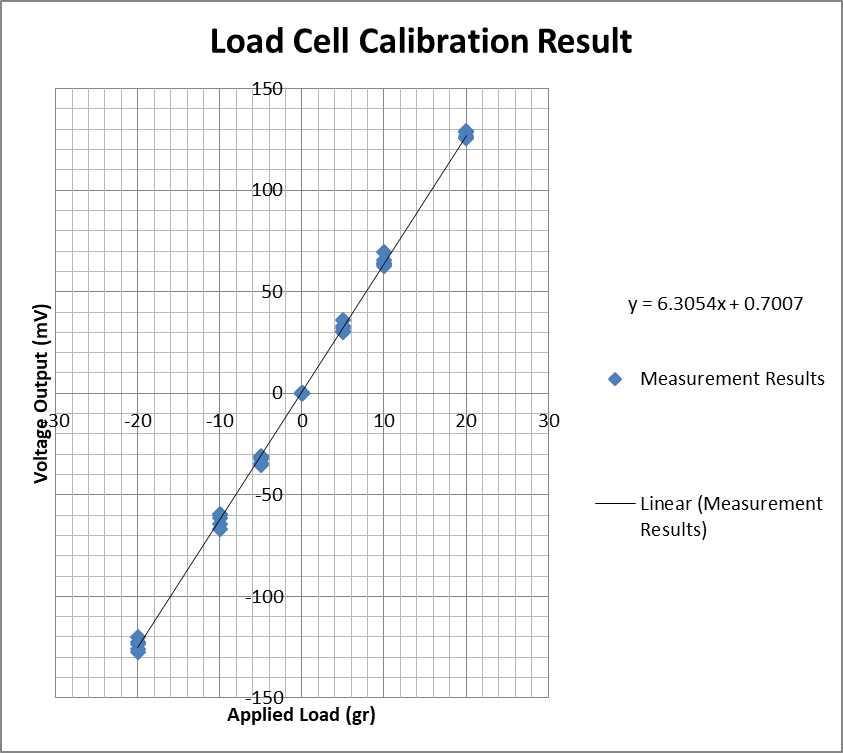
\includegraphics[scale=1]{calibres.png}
    \caption{Load cell calibration result.}
    \label{fig:calibres}
\end{figure}
From linear curve fitting method available in Excel, the relationship between voltage output and applied load can be expressed mathematically as:
\begin{equation}
    V_{o} = 6.3054W_{i} + 0.7007
    \label{eq:calibres}
\end{equation}
\section{Net Thrust Force Optimisation Result}
\label{sec:optimiseresult}
The sample points chosen to be experimentally evaluated was found through Halton sequence algorithm made by Dwianto (2015). This algorithm's output is the normalised stiffener length which served as the sample for this experiment. At each sample, the fin was flapped and moved 5 times in which each experimental runs produce 15 oscillation cycles to ensure repeatability. The net thrust force was the average of force measured in every cycle. After the sampling process is done, the resulting data sets was used to calculate the fitness function using G-SAGA and the predicted optimum value of the data was obtained. This predicted optimum value was then validated by running one more experimental run at the predicted optimum condition. Figure \ref{fig:flowchartmeth} shows the flowchart of this process.\par
\begin{figure}[H]
    \centering
    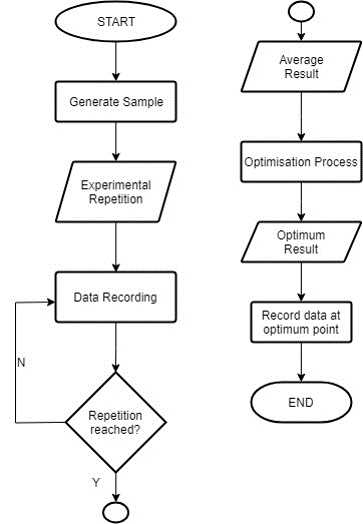
\includegraphics[scale=0.8]{flowchartmeth.png}
    \caption{Optimisation of net thrust flowchart.}
    \label{fig:flowchartmeth}
\end{figure}
Three cases were tested as part of this thesis: stiffness optimisation, stiffness and frequency optimisation, and stiffness and velocity optimisation. Those cases were chosen to observe the effect of stiffness distribution along it's chord on thrust generation and the last two cases were chosen to see the interaction between material properties (i.e. stiffness) and kinematic parameters relevant to flapping fin motion.\par
\subsection{Average Net-Thrust vs Stiffener Length}
To optimise the stiffness of the fin panel, force measurement experiment on a towing tank was conducted on the fin panel. As explained in chapter 3, the stiffness of the fin panel can be adjusted by varying the stiffener length that is embedded in the fin panel. The kinematic parameters that was kept as constant were frequency (1 Hz), amplitude (15$^{0}$), and forward velocity (1 cm/s) while the specimen's stiffness was varied by changing the length of the wire that acted as the stiffener. Figures \ref{fig:charteachrun} and \ref{fig:chartensemble} shows the result of this process.\par
\begin{figure}[H]
    \centering
    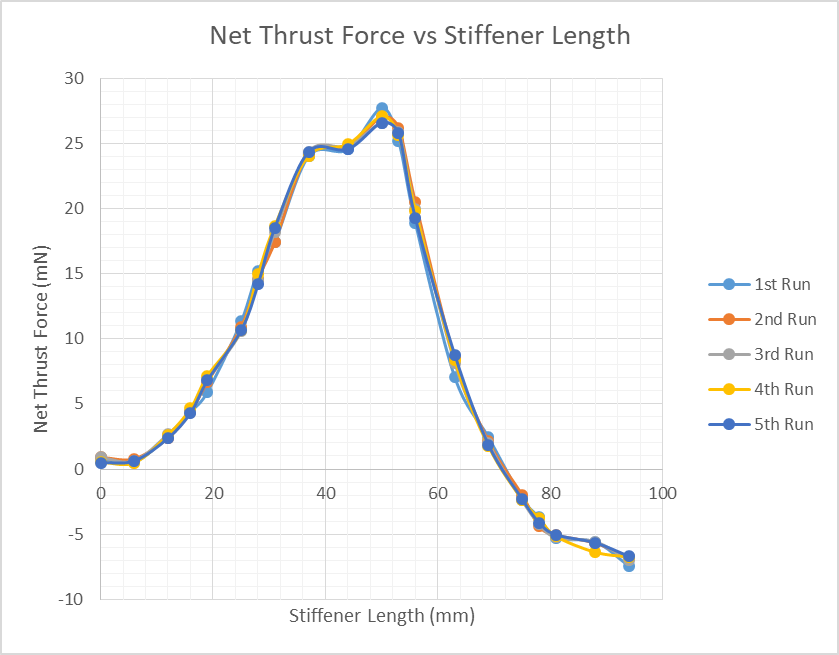
\includegraphics[scale=0.8]{chart_eachrun.png}
    \caption{Net Thrust Force vs Stiffener Length at each experimental runs.}
    \label{fig:charteachrun}
\end{figure}
\begin{figure}[H]
    \centering
    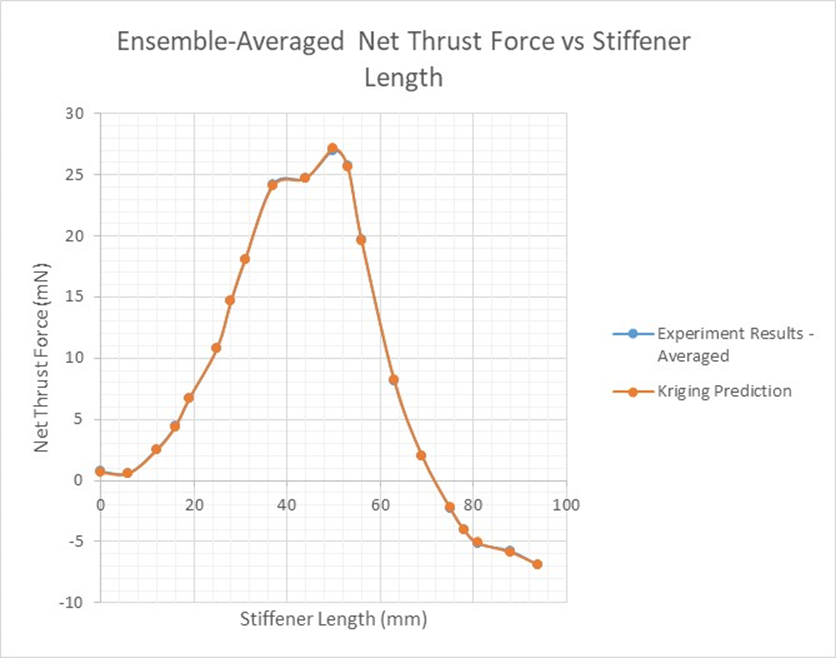
\includegraphics[scale=0.8]{chart_ensemble.png}
    \caption{Ensemble-Averaged Net Thrust Force vs Stiffener Length at each experimental runs.}
    \label{fig:chartensemble}
\end{figure}
Figure \ref{fig:charteachrun} depicts the experimental result over 5 times experimental runs and figure \ref{fig:chartensemble} represents the ensemble-averaged thrust from every experimental runs. From those figures it can be seen that neither the stiffest nor the most flexible fin produce the largest thrust. Instead, it is almost right in the middle, where 50\% wire length produce the largest thrust. It should be noted, however that the predicted thrust from genetic algorithm may very slightly differ from the true experimental result conducted at the exact same stiffener length value. The detailed numbers can be seen in table \ref{tab:tableresult} in which the disrepancies between predicted and true thrust value is almost negligible, also shown in relative error chart with respect to each population depicted in figure \ref{fig:errorfre}. Relative error denoted by $\epsilon$ (Eq. \ref{eq:relerror}) was chosen to quantify the disrepancy between kriging prediction and real experimental result.
\begin{equation}
    \epsilon = 100\% \times \left\lvert 1 - \frac{F_{kriging}}{F_{real}}\right\rvert
    \label{eq:relerror}
\end{equation}
\begin{table}[H]
\centering
\caption{Comparison table between kriging ensembled-averaged thrust force and kriging prediction.}
\vspace{5pt}
\begin{tabular}{|r|r|r|r|r|} 
\hline
No & \begin{tabular}[c]{@{}l@{}}Stiffener Length\\(mm) \end{tabular} & \begin{tabular}[c]{@{}l@{}}Ensemble Average\\(mN)~\end{tabular} & \begin{tabular}[c]{@{}l@{}}Kriging Prediction\\(mN)\\ \end{tabular} & \begin{tabular}[c]{@{}l@{}}Error\\(\%) \end{tabular}  \\ 
\hline
1  & 94                                                              & -7                                                              & -7                                                                  & 0.48                                                  \\ 
\hline
2  & 88                                                              & -6                                                              & -6                                                                  & 1.69                                                  \\ 
\hline
3  & 81                                                              & -5                                                              & -5                                                                  & 1.05                                                  \\ 
\hline
4  & 78                                                              & -4                                                              & -4                                                                  & 0.44                                                  \\ 
\hline
5  & 75                                                              & -2                                                              & -2                                                                  & 1.43                                                  \\ 
\hline
6  & 69                                                              & 2                                                               & 2                                                                   & 2.04                                                  \\ 
\hline
7  & 63                                                              & 8                                                               & 8                                                                   & 1.21                                                  \\ 
\hline
8  & 56                                                              & 20                                                              & 20                                                                  & 0.17                                                  \\ 
\hline
9  & 53                                                              & 26                                                              & 26                                                                  & 0.21                                                  \\ 
\hline
10 & 50                                                              & 27                                                              & 27                                                                  & 0.50                                                  \\ 
\hline
11 & 44                                                              & 25                                                              & 25                                                                  & 0.07                                                  \\ 
\hline
12 & 37                                                              & 24                                                              & 24                                                                  & 0.52                                                  \\ 
\hline
13 & 31                                                              & 18                                                              & 18                                                                  & 0.31                                                  \\ 
\hline
14 & 28                                                              & 15                                                              & 15                                                                  & 0.22                                                  \\ 
\hline
15 & 25                                                              & 11                                                              & 11                                                                  & 0.14                                                  \\ 
\hline
16 & 19                                                              & 7                                                               & 7                                                                   & 0.88                                                  \\ 
\hline
17 & 16                                                              & 4                                                               & 4                                                                   & 1.42                                                  \\ 
\hline
18 & 12                                                    & 3                                                               & 2                                                                   & 2.71                                                  \\ 
\hline
19 & 6                                                               & 1                                                               & 1                                                                   & 6.81                                                  \\ 
\hline
20 & 0                                                               & 1                                                            & 1                                                                   & 11.26                                                 \\
\hline
\end{tabular}
\label{tab:tableresult}
\end{table}
\begin{figure}[H]
    \centering
    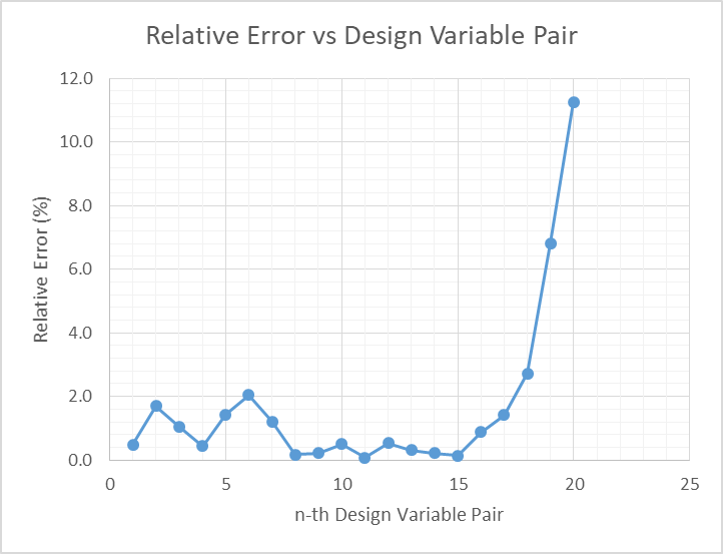
\includegraphics[scale=0.8]{errorstiff.png}
    \caption{Relative Error vs n-th population.}
    \label{fig:errorfre}
\end{figure}
To better understand what happened at each fin, the instantaneous thrust force at three flexibility conditions were presented in figure \ref{fig:chartinstant}. From this figure, it is obvious that the maximum net thrust force produced by fin with 50-50 flexibility produced the highest peak thrust with no force less than zero i.e no drag was present during the motion. However, fully-flexible or fully-stiff fins are not without merit. From the same graph, it can be observed that fully-flexible fin took less time to reached it's peak compared to the fully-stiff fin, the drawback is that while it may be beneficial to increase acceleration, the duration in which the flapping motion produce thrust is less to that of the fully-stiff fin where although it took longer for the fin to reach it's peak, the fin can maintain it's thrust for longer period of time. The same observation was made by Aiello et al. (2018) where it is stated that fish species with stiffer fin tend to produce thrust at longer period of time while flexible fin produce more acceleration at the cost of the fin's propulsion duration.
\label{sec:forceinstant}
\begin{figure}[H]
    \centering
    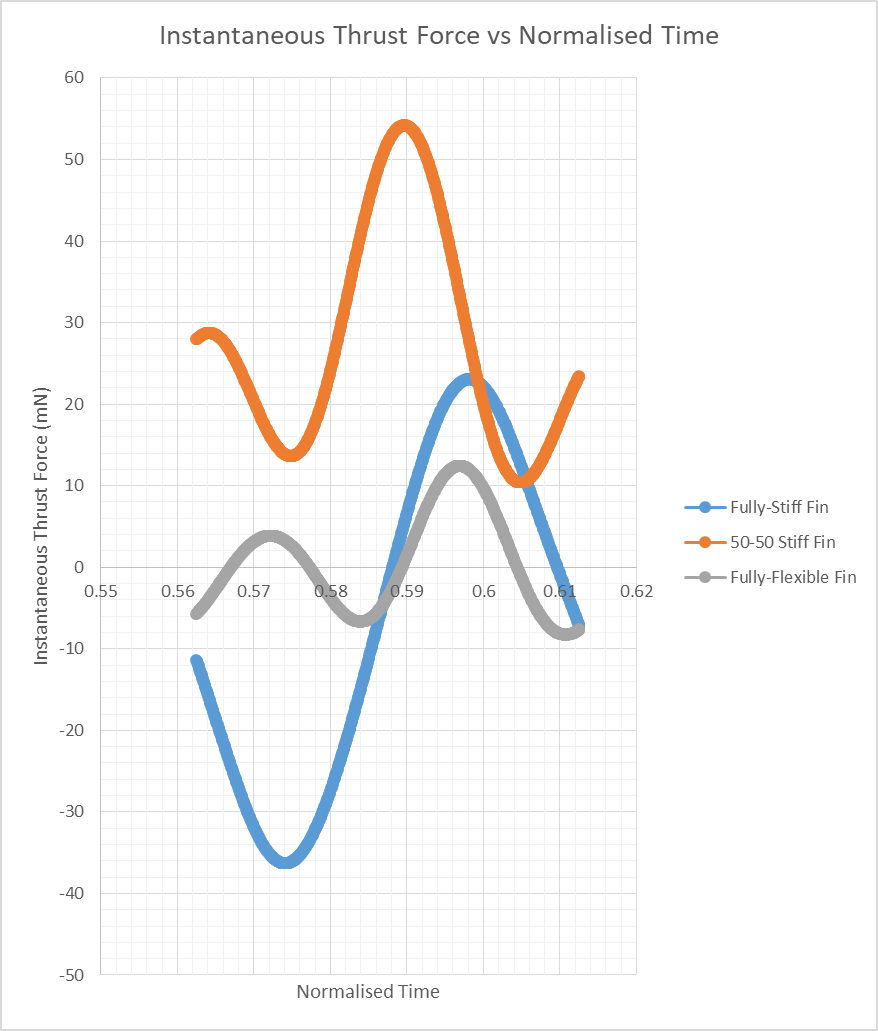
\includegraphics[scale=0.8]{chart_instant.png}
    \caption{Instantaneous Thrust Force vs normalised time.}
    \label{fig:chartinstant}
\end{figure}
\subsection{Average Net-Thrust vs Stiffener Length and Frequency Pair}
In this case, a pair of design variable was tested to find the produced thrust. Stiffener length was chosen from fully-stiff to fully-flexible and the frequency was varied from 0.5 Hz to 2 Hz. This frequency range was chosen due to the fact that the higher the frequency, the servo may not produce the same flapping amplitude as the servo ability to flap the fin was hampered by the fin's own weight. The fin velocity was kept constant at 1 cm/s and the amplitude was also kept constant at 15$^{0}$. This kinematic parameters corresponds to Strouhal number in the range of 0.15 to 0.52.\par
\begin{figure}[H]
    \centering
    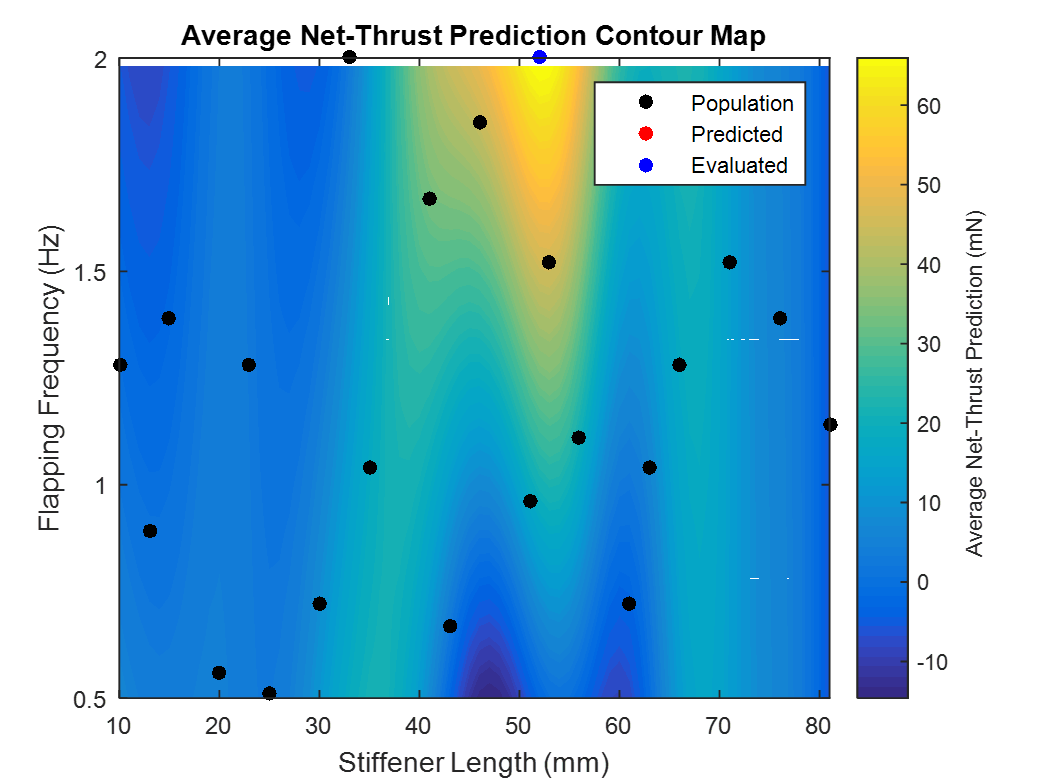
\includegraphics[scale=0.8]{chart_fre.png}
    \caption{Average Net-Thrust Force wrt Stiffener Length and Frequency Contour Map.}
    \label{fig:chart_fre}
\end{figure}
Figure \ref{fig:chart_fre} is the contour maps obtained through kriging interpolation through 21 evaluation at each population denoted by black dots. Through the algorithm, it was obtained that the optimum net-thrust was produced when the stiffness was at 52 mm flapping at 2 Hz frequency. It was predicted that the thrust will produce 67.78 mN. To check whether the prediction was true or not, an experiment was run at the predicted optimum condition which yield 68 mN net-thrust, making the relative error very small at 0.4\%, which indicates that the kriging prediction accurately predicts the average net-thrust given the stiffener length and flapping frequency. The detailed result of each population evaluation is expressed in table \ref{tab:tableresultfre} and the relative error graph can be seen in figure \ref{fig:errorfre}.
\begin{table}[H]
\centering
\caption{Comparison table between kriging ensembled-averaged thrust force and kriging prediction -- stiffness and flapping frequency combination.}
\vspace{5pt}
\begin{tabular}{|l|l|l|l|l|l|} 
\hline
\multirow{2}{*}{No} & \multicolumn{2}{c|}{Sample}                                                                                                       & \multicolumn{2}{c|}{\begin{tabular}[c]{@{}l@{}}Net-Thrust Average\\(mN) \end{tabular}} & \multirow{2}{*}{\begin{tabular}[c]{@{}l@{}}Relative Error\\(\%)~\end{tabular}}  \\ 
\cline{2-5}
                    & \begin{tabular}[c]{@{}l@{}}Stiffener Length\\(mm)\end{tabular} & \begin{tabular}[c]{@{}l@{}}Flapping Frequency\\(mN)\end{tabular} & Evaluated & Predicted                                                                   &                                                                                 \\ 
\hline
1                   & 81                                                             & 1.14                                                             & -6        & -6                                                                          & 6.6                                                                             \\ 
\hline
2                   & 76                                                             & 1.39                                                             & 6         & 6                                                                           & 6.0                                                                             \\ 
\hline
3                   & 71                                                             & 1.52                                                             & 14        & 14                                                                          & 0.0                                                                             \\ 
\hline
4                   & 66                                                             & 1.28                                                             & 18        & 18                                                                          & 2.2                                                                             \\ 
\hline
5                   & 63                                                             & 1.04                                                             & 7         & 7                                                                           & 1.1                                                                             \\ 
\hline
6                   & 61                                                             & 0.72                                                             & -3        & -3                                                                          & 10.9                                                                            \\ 
\hline
7                   & 56                                                             & 1.11                                                             & 21        & 21                                                                          & 0.9                                                                             \\ 
\hline
8                   & 53                                                             & 1.52                                                             & 46        & 46                                                                          & 0.7                                                                             \\ 
\hline
9                   & 52                                                             & 2.00                                                             & 68        & 68                                                                          & 0.3                                                                             \\ 
\hline
10                  & 51                                                             & 0.96                                                             & 17        & 17                                                                          & 2.4                                                                             \\ 
\hline
11                  & 46                                                             & 1.85                                                             & 44        & 44                                                                          & 0.2                                                                             \\ 
\hline
12                  & 43                                                             & 0.67                                                             & 3         & 3                                                                           & 1.5                                                                             \\ 
\hline
13                  & 41                                                             & 1.67                                                             & 33        & 33                                                                          & 0.2                                                                             \\ 
\hline
14                  & 35                                                             & 1.04                                                             & 18        & 18                                                                          & 0.4                                                                             \\ 
\hline
15                  & 33                                                             & 2.00                                                             & 3         & 3                                                                           & 8.5                                                                             \\ 
\hline
16                  & 30                                                             & 0.72                                                             & 9         & 9                                                                           & 4.0                                                                             \\ 
\hline
17                  & 25                                                             & 0.51                                                             & 3         & 3                                                                           & 2.4                                                                             \\ 
\hline
18                  & 23                                                             & 1.28                                                             & 3         & 3                                                                           & 4.3                                                                             \\ 
\hline
19                  & 20                                                             & 0.56                                                             & 5         & 5                                                                           & 1.3                                                                             \\ 
\hline
20                  & 15                                                             & 1.39                                                             & -2        & -2                                                                          & 2.4                                                                             \\ 
\hline
21                  & 13                                                             & 0.89                                                             & 1         & 1                                                                           & 17.8                                                                            \\ 
\hline
22                  & 10                                                           & 1.28                                                             & 0         & 0                                                                           & 100.0                                                                           \\
\hline
\end{tabular}
\label{tab:tableresultfre}
\end{table}
\begin{figure}[H]
    \centering
    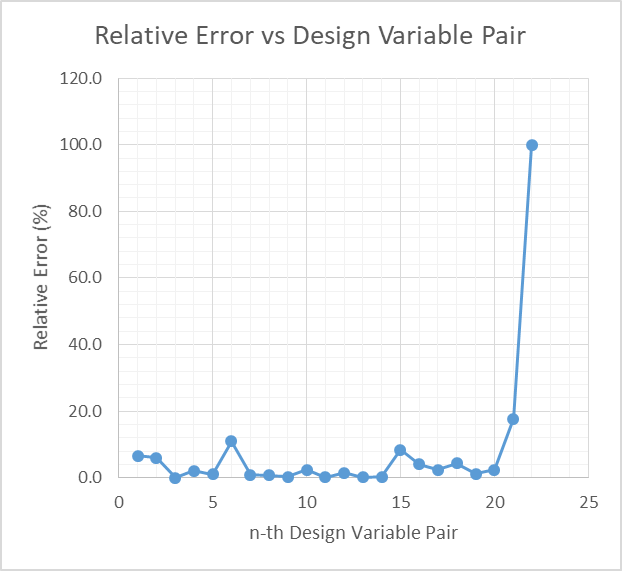
\includegraphics[scale=0.8]{errorfre.png}
    \caption{Relative Error vs n-th population -- Stiffness and Flapping Frequency Combination.}
    \label{fig:errorfre}
\end{figure}
From the relative error graph it can be seen that the kriging prediction error never exceeds 10\%, except at 22nd sample pair. This isn't to say that the kriging prediction is not globally accurate, rather the compared value (the denominator in the relative error calculation) is very close to zero, resulting in very large result, eventhough it was demonstrated that the disrepancy between the predicted average net-thrust value with the measured value is very small.
\subsection{Average Net-Thrust vs Stiffener Length and Velocity Pair}
Similar with the second case, a pair of design variable was tested to find the produced thrust. This time, the chosen kinematics parameter was forward velocity. Again, stiffener length was chosen from fully-stiff to fully-flexible while the velocity was varied from 0.15 cm/s to 4 cm/s. This velocity range was chosen to find the largest Strouhal number range possible given the experimental setup, as the faster the velocity, the more time it took to obtain 15 oscillation cycles, which means the displacement needed is also larger which was bounded by the length of the experimental setup. The fin frequency was kept constant at 1 Hz and the amplitude was also kept constant at 15$^{0}$. This kinematic parameters corresponds to Strouhal number in the range of 0.07 to 1.85.\par
\begin{figure}[H]s
    \centering
    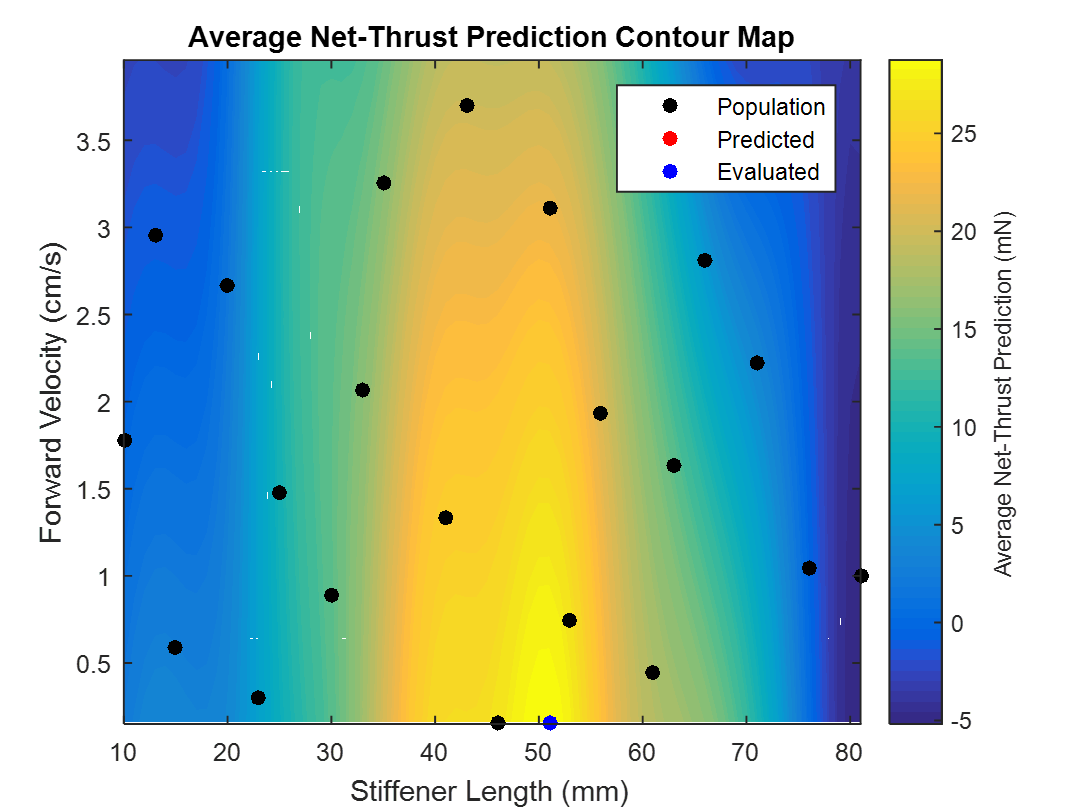
\includegraphics[scale=0.8]{chart_velo.png}
    \caption{Average Net-Thrust Force wrt Stiffener Length and Velocity Contour Map.}
    \label{fig:chart_velo}
\end{figure}
Figure \ref{fig:chart_velo} is the contour maps obtained through kriging interpolation through 21 evaluation at each population denoted by black dots. Through the algorithm, it was obtained that the optimum net-thrust was produced when the stiffness was at 51 mm moving forward at 0.16 cm/s and the predicted average net-thrust was 29.08 mN while the measured average net-thrust at the predicted optimum condition was 29 mN, resulting in an insignificant relative error: 0.3\%. This implies that the kriging prediction accurately predicts the average net-thrust given the stiffener length and forward velocity. The detailed result of each population evaluation is expressed in table \ref{tab:tableresultvelo} and the relative error graph can be seen in figure \ref{fig:errorvelo}.
\begin{table}[H]
\centering
\caption{Comparison table between kriging ensembled-averaged thrust force and kriging prediction -- stiffness and forward velocity combination.}
\vspace{5pt}
\begin{tabular}{|l|l|l|l|l|l|} 
\hline
\multirow{2}{*}{No} & \multicolumn{2}{c|}{Sample}                                                                                                       & \multicolumn{2}{c|}{\begin{tabular}[c]{@{}l@{}}Net-Thrust Average\\(mN) \end{tabular}} & \multirow{2}{*}{\begin{tabular}[c]{@{}l@{}}Relative Error\\(\%)\end{tabular}}  \\ 
\cline{2-5}
                    & \begin{tabular}[c]{@{}l@{}}Stiffener Length\\(mm)\end{tabular} & \begin{tabular}[c]{@{}l@{}}Forward Velocity\\(cm/s)\end{tabular} & Evaluated & Predicted                                                                   &                                                                                 \\ 
\hline
1                   & 81                                                             & 1.00                                                             & -5        & -5                                                                          & 2.4                                                                             \\ 
\hline
2                   & 76                                                             & 1.04                                                             & 0         & 0                                                                           & 100.0                                                                           \\ 
\hline
3                   & 71                                                             & 2.22                                                             & 4         & 4                                                                           & 3.4                                                                             \\ 
\hline
4                   & 66                                                             & 2.81                                                             & 6         & 6                                                                           & 5.8                                                                             \\ 
\hline
5                   & 63                                                             & 1.63                                                             & 14        & 14                                                                          & 0.4                                                                             \\ 
\hline
6                   & 61                                                             & 0.44                                                             & 18        & 18                                                                          & 1.2                                                                             \\ 
\hline
7                   & 56                                                             & 1.93                                                             & 21        & 21                                                                          & 0.8                                                                             \\ 
\hline
8                   & 53                                                             & 0.74                                                             & 27        & 27                                                                          & 0.9                                                                             \\ 
\hline
9                   & 51                                                             & 0.16                                                             & 29        & 29                                                                          & 0.3                                                                             \\ 
\hline
10                  & 51                                                             & 3.11                                                             & 22        & 22                                                                          & 1.4                                                                             \\ 
\hline
11                  & 46                                                             & 0.15                                                             & 27        & 27                                                                          & 1.6                                                                             \\ 
\hline
12                  & 43                                                             & 3.70                                                             & 20        & 20                                                                          & 0.2                                                                             \\ 
\hline
13                  & 41                                                             & 1.33                                                             & 25        & 25                                                                          & 1.0                                                                             \\ 
\hline
14                  & 35                                                             & 3.26                                                             & 16        & 16                                                                          & 3.0                                                                             \\ 
\hline
15                  & 33                                                             & 2.07                                                             & 16        & 16                                                                          & 3.1                                                                             \\ 
\hline
16                  & 30                                                             & 0.89                                                             & 14        & 14                                                                          & 3.1                                                                             \\ 
\hline
17                  & 25                                                             & 1.48                                                             & 10        & 10                                                                          & 4.6                                                                             \\ 
\hline
18                  & 23                                                             & 0.30                                                             & 7         & 7                                                                           & 1.3                                                                             \\ 
\hline
19                  & 20                                                             & 2.67                                                             & 2         & 2                                                                           & 4.8                                                                             \\ 
\hline
20                  & 15                                                             & 0.59                                                             & 3         & 3                                                                           & 4.1                                                                             \\ 
\hline
21                  & 13                                                             & 2.96                                                             & -1        & -1                                                                          & 65.8~ ~ ~ ~ ~~                                                                  \\ 
\hline
22                  & 10                                                        & 1.78                                                        & 0         & 0                                                                           & 100.0~~                                                                         \\
\hline
\end{tabular}
\label{tab:tableresultvelo}
\end{table}
\begin{figure}[H]
    \centering
    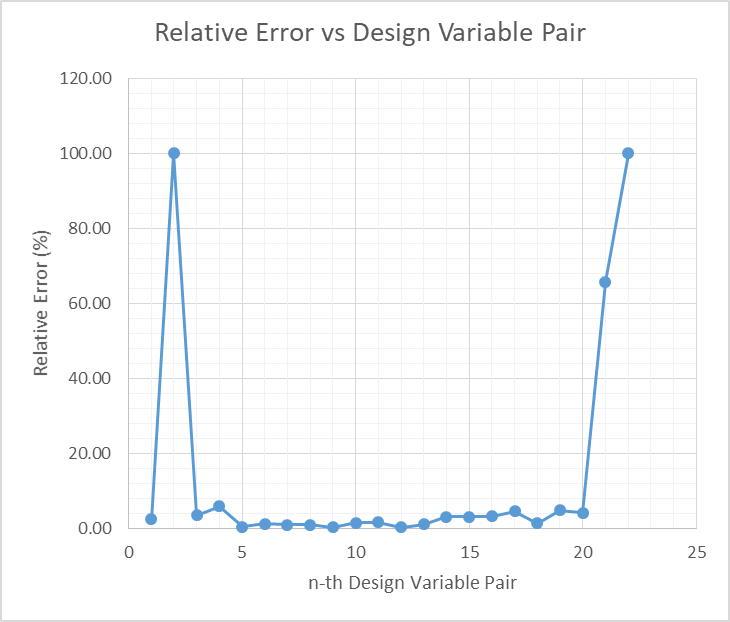
\includegraphics[scale=0.8]{errorvelo.png}
    \caption{Relative Error vs n-th population.}
    \label{fig:errorvelo}
\end{figure}
From the relative error graph it can be seen that the kriging prediction error never exceeds 10\%, except at 2nd, 21st, and 22nd sample pairs. As with the result from the frequency and stiffness measurement, the reason for this seemingly large error isn't that the kriging prediction is inaccurate, it is rather due to the compared value (the denominator in the relative error calculation) is very close to zero in the 2nd and 22nd case, and very close to -1 in the 21st sample pair case which results in a very large result, eventhough difference between the predicted average net-thrust value with the measured value is very small.
\section{Result Discussion and Analysis}
\label{sec:discuss}
Before delving deeper into the analysis of the results shown in \ref{sec:optimiseresult}, it is appropriate to first discuss whether the results obtained from the experiment is acceptable or not. One of the main difference between experimental method and computational or analytical method is that the result that one obtains may or may not be the accurate result. Unlike computational or analytical method where the same output is guaranteed given the same process and the same input, experimental method output can vary due to, for example, the existence of random noise during the experiment and the measuring instruments sensitivity. Therefore, it is important to make sure that the result obtained from experiment is the right result, or in other words, it is important to ensure the repeatability of the experimental result. The concrete value that can be used to measure the repeatability of an experiment given a set of sample $N$ of an observed variable $x$ is standard deviation depicted as $s$ (Eq. \ref{eq:stdev}) or standard deviation of the mean, represented as $s_{m}$ (Eq. \ref{eq:stdevmean}). In this thesis, the standard deviation of the mean was chosen because the value that was analysed in this thesis is the average of a value (net thrust).\par
\begin{equation}
    s = \sqrt{\frac{1}{N-1} \sum_{i=1}^N (x_i - \overline{x})^2}
    \label{eq:stdev}
\end{equation}
\begin{equation}
    s_{m} = \frac{s}{\sqrt{N}}
   \label{eq:stdevmean}
\end{equation}
\begin{table}[H]
\centering
\caption{Standard deviation of the mean for each experimental result.}
\vspace{5pt}
\begin{tabular}{|l|l|l|l|} 
\hline
\multirow{2}{*}{No} & \multicolumn{3}{l|}{\begin{tabular}[c]{@{}l@{}}Standard Deviation\\of the Mean\end{tabular}}  \\ 
\cline{2-4}
                    & Case I                             & Case II & Case II                                        \\ 
\hline
1                   & 0.14                               & 0.14    & 0.20                                           \\ 
\hline
2                   & 0.15                               & 0.20    & 0.20                                           \\ 
\hline
3                   & 0.05                               & 0.22    & 0.37                                           \\ 
\hline
4                   & 0.13                               & 0.09    & 0.24                                           \\ 
\hline
5                   & 0.07                               & 0.12    & 0.07                                           \\ 
\hline
6                   & 0.12                               & 0.18    & 0.12                                           \\ 
\hline
7                   & 0.30                               & 0.03    & 0.25                                           \\ 
\hline
8                   & 0.28                               & 0.23    & 0.08                                           \\ 
\hline
9                   & 0.16                               & 0.24    & 0.08                                           \\ 
\hline
10                  & 0.21                               & 0.11    & 0.27                                           \\ 
\hline
11                  & 0.08                               & 0.32    & 0.08                                           \\ 
\hline
12                  & \textcolor[rgb]{0.2,0.2,0.2}{0.07} & 0.21    & 0.40                                           \\ 
\hline
13                  & \textcolor[rgb]{0.2,0.2,0.2}{0.26} & 0.16    & 0.23                                           \\ 
\hline
14                  & \textcolor[rgb]{0.2,0.2,0.2}{0.18} & 0.07    & 0.08                                           \\ 
\hline
15                  & \textcolor[rgb]{0.2,0.2,0.2}{0.14} & 0.14    & 0.11                                           \\ 
\hline
16                  & \textcolor[rgb]{0.2,0.2,0.2}{0.21} & 0.14    & 0.08                                           \\ 
\hline
17                  & \textcolor[rgb]{0.2,0.2,0.2}{0.06} & 0.08    & 0.05                                           \\ 
\hline
18                  & \textcolor[rgb]{0.2,0.2,0.2}{0.06} & 0.08    & 0.16                                           \\ 
\hline
19                  & \textcolor[rgb]{0.2,0.2,0.2}{0.05} & 0.13    & 0.08                                           \\ 
\hline
20                  & \textcolor[rgb]{0.2,0.2,0.2}{0.09} & 0.04    & 0.16                                           \\
\hline
\end{tabular}
\label{tab:stddevofmean}
\end{table}
Table \ref{tab:stddevofmean} shows the standard error of the mean of each cases that was run in this thesis. Ideally, SDM close to zero is desirable as it means that the variance of the data is minimum. It is shown that the SDM of each population is less than 0.5, which leads to the conclusion that the result obtained from the experiment was indeed the right result and five experimental results are enough to obtain data point with minimum variance.\par
The changing of the fin's stiffener length (therefore it's effective stiffness) resulted in the change of thrust produced by the fin. This result is consistent with \citet{Esposito56}. From the same research, it was also shown that neither the stiffest nor the most flexible fin produce the highest thrust; instead the highest thrust was produced when the fin's stiffness was stiffer towards the leading edge up until the mid-chord and flexible from the mid-chord towards the trailing edge. Interestingly enough, this configuration holds across different kinematic parameters variation. The reason for this result was due to the nature of flapping-based thrust generation: when the fin accelerated, fluid is pushed along it's symmetrical axis and the thrust is gradually increasing as the fin goes from the extreme lateral position (i.e it's flapping amplitude). When the fin reached mid-stroke, the thrust force peaked and gradually decrease until at some point, depending on the kinematical and material properties, becomes drag \citep{Esposito56,zhushoele,akhtar}. From this argument it can then be inferred that the larger the amplitude -- therefore the lateral displacement -- the larger the thrust. This argument is backed from previous result by \citet{luqman} and \citet{hiroki} where half-stiff half-flexible fin produce the largest lateral displacement due to the difference of bending modes in various fin stiffness (see Figure \ref{fig:luqmandisp}). If the fin is fully flexible, the resulting fin shape at it's extreme amplitude is not fully deflected toward either side, instead the fin produce camber-like profile which in turn resulting in smaller lateral displacement. If the fin is fully stiff, the resulting deflection does not produce larger displacement as the fin with 50-50 stiffness.\par
\begin{figure}[H]
    \centering
    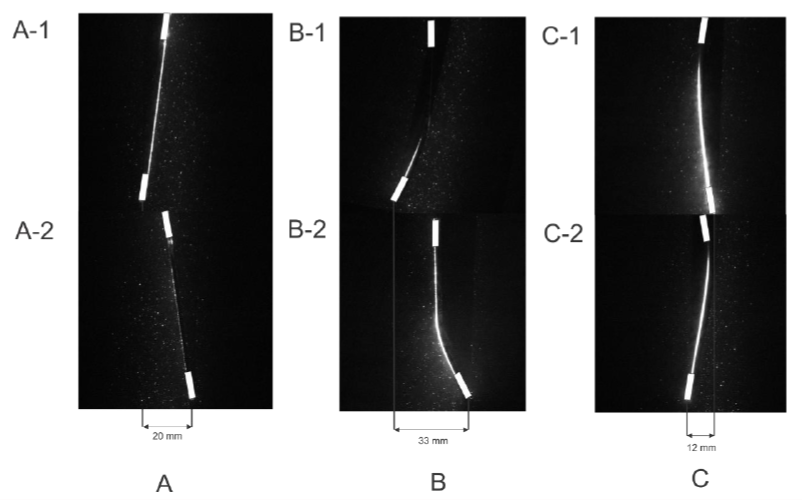
\includegraphics[scale=0.5]{luqman_disp.png}
    \caption{Real pictures captured at each extreme lateral displacement. (A) Fin number 1, (B) fin number 4, and (C) fin number 7. Upper part shows positive angle of stroke and lower one shows negative angle of stroke. Adapted from Fathurrohim (2016).}
    \label{fig:luqmandisp}
\end{figure}
\citet{aiello} also argued that this configuration (i.e stiffer at the leading edge and flexible at the trailing edge) leads to bending resistance caused by inertial and hydrodynamics forces acting on the fin where these two forces are associated with propursol reversal between the upstroke and downstroke. It is also argued that stiffened leading edge and flexible trailing edge results in propeller-like twist as a response to the torsional force, as argued by \citet{wootton} by observing that insect generates a camberline across the wing \citep{ennos}. Camber generation due to the stiffness can increase fluid dynamics efficiency and also bending resistance.\par
Frequency variation is by far the most interesting set of data. Firstly, it increased the net-thrust dramatically -- up to nearly 50\% -- which indicates that the average net-thrust change is sensitive to frequency change. Secondly, the same stiffness or frequency change does not produce predictable average net-thrust result. Eventhough 50 mm stiffener length configuration produce the largest thrust across the whole observed domain, the same cannot be said for low frequency condition where 50 mm stiffener length actually does not produce thrust at all. Rather, the lower stiffness configuration yields the most satisfying result given a particular low frequency (less than 1 Hz), as seen in figure \ref{fig:chart_surfre}.
\begin{figure}[H]
    \centering
    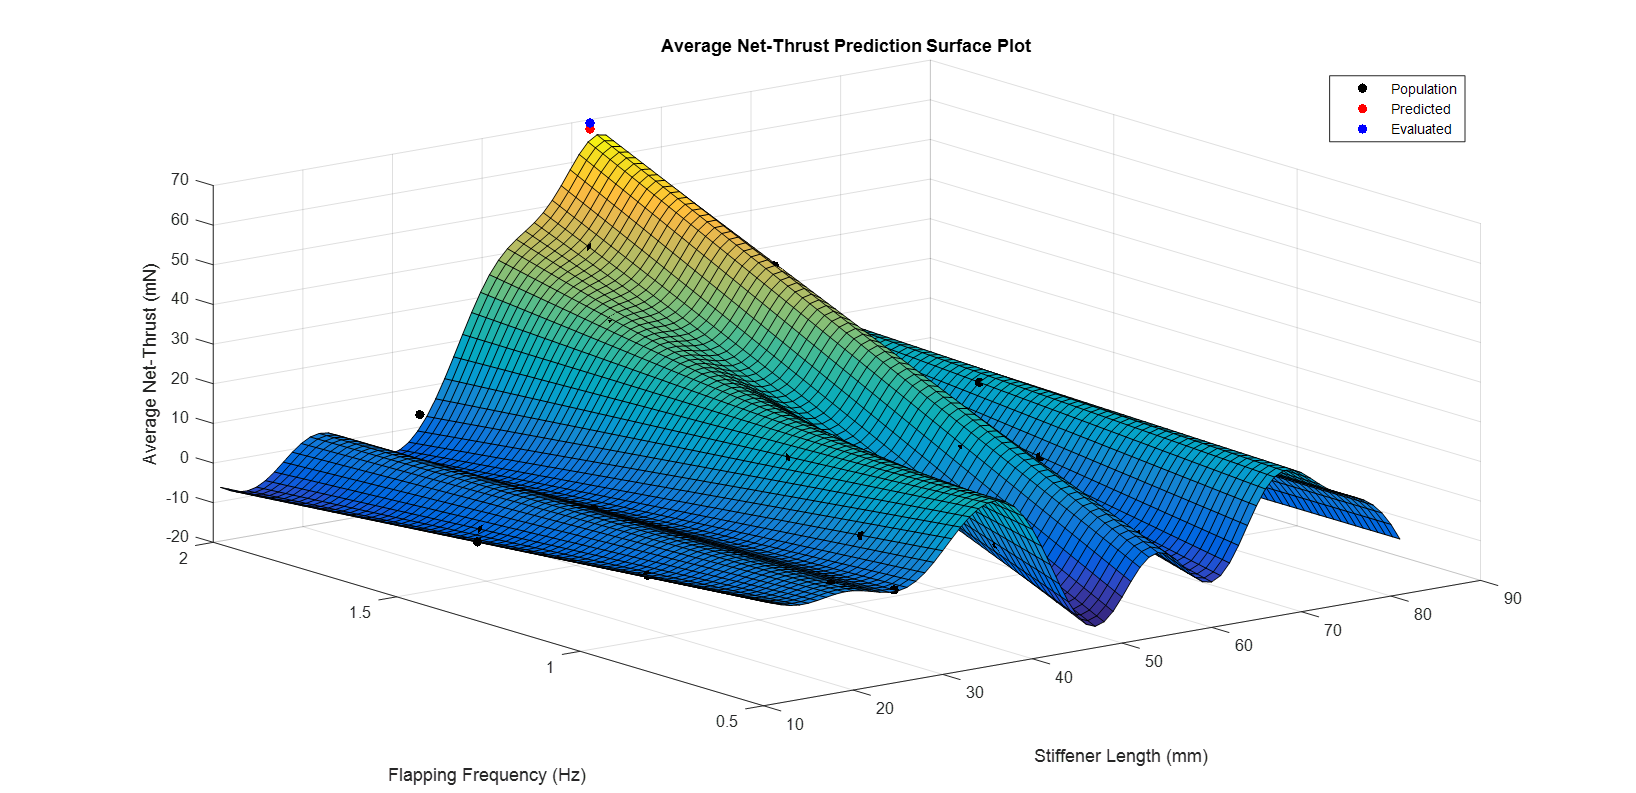
\includegraphics[scale=0.6]{chart_surfre.png}
    \caption{Average Net-Thrust Force wrt Stiffener Length and Frequency Surface Plot.}
    \label{fig:chart_surfre}
\end{figure}
This seemingly unpredictable nature of frequency change is explained by this: for each material configuration, there exist different responses for a given input. In this case, the resulting bending mode is influenced by the input frequency imposed on the fin. This different bending mode leads to smaller or larger trailing edge displacement, which directly influence the strength of the Karman vortex street behind the fin, which is the main ingredients of thrust generation through flapping mechanism. It is possible that at lower frequency, the 50 mm stiffener configuration does not produce as large of amplitude as the lower stiffness configuration, which results in lower thrust output. The same observation was made by \citet{Esposito56}, further validating this analysis.\par
Multiple interesting observations from the change of velocity variation experiment are two things: first, change of velocity and stiffness results in a somewhat uniform change in average net-thrust i.e. as the velocity decrease, the average net-thrust increase while the change of stiffness does not affect the net-thrust generation as much as the change in frequency, demonstrated in the surface plot of the average net-thrust vs flapping velocity and fin stiffness (Figure \ref{fig:chart_survelo}).
\begin{figure}[H]
    \centering
    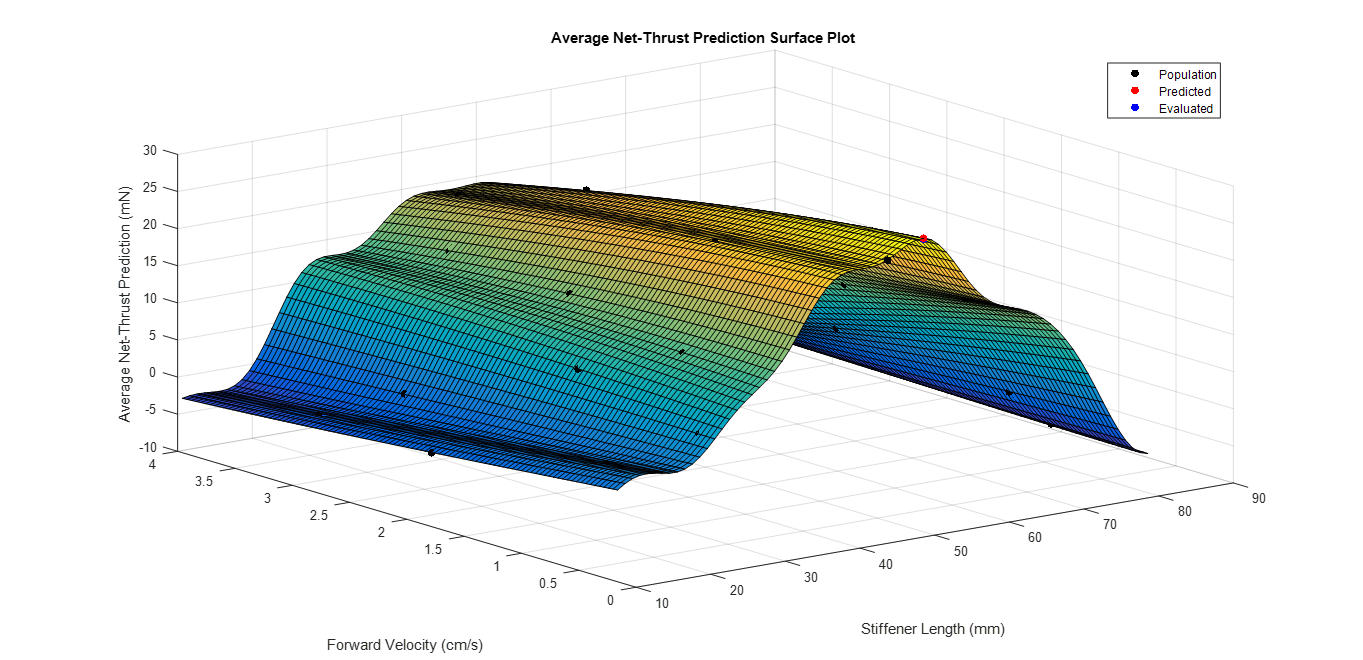
\includegraphics[scale=0.6]{chart_survelo.png}
    \caption{Average Net-Thrust Force wrt Stiffener Length and Velocity Surface Plot.}
    \label{fig:chart_survelo}
\end{figure}
This can be explained by two things: first is that aerodynamics dictates that the larger the velocity, the greater the drag force. This increase in drag force accompanying velocity increase results in the decrease in the instaneous thrust generated by the flapping fin, which leads to the decrease in the average net-thrust. Another explanation is that the nature of thrust generation through the flapping mechanism itself. From chapter II it was outlined that the thrust generated by flapping mechanism relies on the generation of reversed Karman street vortex. The reverse in vortex direction can only be achieved if the velocity combined with the flapping frequency (i.e. Strouhal number) is such that the flow around the fin produce this reverse in vortex direction. If the velocity is large enough and the frequency is small enough, the resulting vortex around the fin does not produce strong enough vortex to create a meaningful induced-velocity at the aft of the fin, which is essential to thrust generation. In some cases, as observed in the first and 21st stiffness-frequency pair, the resulting net-thrust is actually negative i.e. this configuration produces drag instead. This result arised from the fact that at this configuration, instead of the fin produced a reversed Karman vortex street, it produced an unreversed Karman vortex street which behaves similarly as if a blunt body is moving through a freestream. Another observation is that the change in velocity only results in about 6\% increase of net-thrust, compared to the nearly 150\% increase in net-thrust produced by frequency variation. This indicates that net-thrust change is not sensitive to velocity variation, as also shown by \citet{hiroki}, solidifying the analysis given in this thesis.\par

% This is where to put your conclusions and possible future works. Write it in chapters/bab5.tex
\chapter{Conclusion and Future Works}
\section{Conclusion}
G-SAGA with kriging has been implemented succesfully to predict the optimum flexibility distribution across the fin's spanwise direction, with error never exceeding 10\% for all populations tested. There also exist a significant relationship between fin flexibility and the generated thrust, which holds true for different kinematical parameters tested. The reason for this relationship is that different bending modes related to flexibility resulted in higher lateral movement of the fin's trailing edge which in turm produce higher lateral separation between the Reversed-Karman vortex sheet. Flexibility distribution also affects the resistance of the fin to bending produced by inertial and hydrodynamical forces exerted to the fin, which has been associated with propulsor reversal phenomena in-between strokes. Different bending mode is also responsible to the existence of camber along the fin, making the fin's profile similar to that of traditional propellers which resulted in increase of fluid dynamics efficiency. Another observation is that frequency plays a larger role to thrust generation compared to velocity as the increase of net-thrust average due to frequency change is close to 50\%, compared to increase of net-thrust by changing the velocity: 6\%. However, the effect of bending modes also plays a role in frequency variation, as the most optimum configuration does not yield optimum result given a specific frequency, particularly at lower frequency, due to different frequency produce different chord-wise profile as a response to the given frequency. 
\section{Future Works}
The future sequel to this work may include:
\begin{enumerate}
    \item Flow visualisation of the wake structure behind the fin.

    While there are a lot of previous researches that delves into the effect of fin flexibility to thrust generation visually, it will be interesting to observe the wake structure behind the fin to better understand the mechanism of thrust generation associated with flexibility.
    \item Checking the optimum kinematical parameters for different fin stiffness.

    Different fin stiffness produce different results which might indicates that for every stiffness configuration, there exist an optimum swimming condition for a given fin stiffness.
    \item Study the three dimensionality effect of thrust generation

    It is argued that it is not the stiffness of a fin that relates to thrust generation, instead it is the flexural flexibility (multiplication of second moment of inertia with Young's modulus) that is related to the thrust. It may be interesting to see the effect of moment of inertia and finding the optimum value of the moment of inertia, which indirectly relates to optimising the shape of the fin instead of using simple rectangle fin.
\end{enumerate}

% Bibliography. It should be printed automatically. Make sure to run bibtex on mythesis.aux and recompile mythesis.tex
\printbibliography[heading=bibintoc,title=References]

% This is the appendix part. Put your pseudocode and the like here.
\chapter*{Appendix}
\addcontentsline{toc}{chapter}{Appendix}
\lstset{
    language=Matlab,%
    basicstyle=\ttfamily,
    breaklines=true,%
    keywordstyle=\color{blue},%
    identifierstyle=\color{black},%
    stringstyle=\color{yellow},
    commentstyle=\color{green},%
    showstringspaces=false,%without this there will be a symbol in the places where there is a space
    numbers=left,%
    numberstyle={\tiny \color{black}},% size of the numbers
    numbersep=9pt, % this defines how far the numbers are from the text
    emph=[1]{for,end,break},emphstyle=[1]\color{red}, %some words to emphasise
    %emph=[2]{word1,word2}, emphstyle=[2]{style},    
}
\begin{lstlisting}[caption={Pseudocode for main DAQ Code in MATLAB}]
clc
clear all
close all

%% INITIALISING
b = 0.0018;
m = 6.92;

ai = daq.createSession('ni');
addAnalogInputChannel(ai,'Dev2', 'ai0', 'Voltage');
ai.Rate = 500;

disp('Calculating zero load balance...');

[data,time] = ai.startForeground;

zerobal = mean(data);

disp('Begin the flapping motion in Arduino!')
pause(8);

%% DATA COLLECTING
disp('Collecting data...');

ai.DurationInSeconds = 13;

[volt,time] = ai.startForeground;

volt = (volt - zerobal)*1E3;
forceNormal = (volt - b)/m*9.81*1E-3;

%% FILTERING & SMOOTHING
% Filter design using 4th order Butterworth filter 
n = 4;
cutoffFreq = 2;
wn = 2*cutoffFreq/ai.Rate;
[z,p] = butter(n,wn);

% Actual filtering process
filterVolt = filter(z,p,volt);
filterforceNormal = filter(z,p,forceNormal);

% Smoothing process using moving average method up to 100 pts forward
smoothforceNormal = smooth(filterforceNormal,500,'moving');
forceAverage = mean(smoothforceNormal);

%% PLOTTING
figures = plot(time,smoothforceNormal);
xlabel('Time (s)');
ylabel('Normal Force (N)');
grid on;

%% SAVING
evalCase = 1;
save(['Experiment_Result',num2str(evalCase),'.mat'],'time','smoothforceNormal');
savefig(['Experiment_Result',num2str(evalCase),'.fig'],'figures');
\end{lstlisting}

\lstset{
    language=C++,%
    basicstyle=\ttfamily,
    breaklines=true,%
    keywordstyle=\color{blue}\ttfamily,
    stringstyle=\color{red}\ttfamily,
    commentstyle=\color{green}\ttfamily,
    morecomment=[l][\color{magenta}]{\#}
    showstringspaces=false,%without this there will be a symbol in the places where there is a space
    numbers=left,%
    numberstyle={\tiny \color{black}},% size of the numbers
    numbersep=9pt, % this defines how far the numbers are from the text
    emph=[1]{for,end,break},emphstyle=[1]\color{red}, %some words to emphasise
    %emph=[2]{word1,word2}, emphstyle=[2]{style},    
}
\begin{lstlisting}[caption={Code for traversing module in Arduino}]
  /* Sweep
  by BARRAGAN <http://barraganstudio.com>
  This example code is in the public domain.

  modified 8 Nov 2013
  by Scott Fitzgerald
  http://www.arduino.cc/en/Tutorial/Sweep

  Modified 7 Jul 2018
  by MI
  change delay to millis()
*/

#include <Servo.h>
#include <AccelStepper.h>

Servo myServo;
AccelStepper myStepper (1, 10, 11);

const int servoMinDegrees = 75;
const int servoMaxDegrees = 105;
const int servoCenterDegree = 90;
const int servoPin = 9;
const int stepperPulsePin = 10;
const int stepperDirPin = 11;

float servoPosition = 90;
/*
 * Set frequency in servoInterval
 * servoInterval = 8.325/desiredFrequency
 */
int servoInterval = 8;
float servoDegrees = 1;

unsigned long timeInit, timeFinal, timeElapsed;
unsigned long currentMillis = 0;
unsigned long previousServoMillis = 0;

void setup() {
  myServo.attach(servoPin);
  myServo.write(servoPosition);
  myStepper.setMaxSpeed(6000);

  Serial.begin(9600);// rate at which the arduino communicates
  Serial.println("TOWING TANK 2.0 MOTION MODULE");
}

void loop() {
  /*
   * Options: put 1, 2, or 3
     1. Flapping forward (moving away from user)
     2. Backward w/o flapping (moving toward user)
     3. Centering
  */
  int option = 1;
  if (option == 1) {
    currentMillis = millis();
    rotateStepperForward();
    rotateServo();
  }
  else if (option == 2) {
    rotateStepperBackward();
  }
  else if (option == 3) {
    myServo.write(servoCenterDegree);
  }
}

void rotateStepperForward() {
  /*
   * moveTo(8000) = 10 cm
   * setSpeed(800) = 1 cm/s
   */
  if (myStepper.distanceToGo() == 0) {
    myStepper.moveTo(8000);
    myStepper.setSpeed(800);
  }
  myStepper.runSpeedToPosition();
}

void rotateStepperBackward() {
  if (myStepper.distanceToGo() == 0) {
    myStepper.moveTo(-8000);
    myStepper.setSpeed(800);
  }
  myStepper.runSpeedToPosition();
}

void rotateServo() {
  /*
    This is similar to the servo sweep example except that it uses millis() rather than delay()
    nothing happens unless the interval has expired
    the value of currentMillis was set in loop()
  */
  if (currentMillis - previousServoMillis >= servoInterval) {
    // its time for another move
    previousServoMillis += servoInterval;

    servoPosition = servoPosition + servoDegrees; // servoDegrees might be negative

    if ((servoPosition >= servoMaxDegrees) || (servoPosition <= servoMinDegrees))  {
      // if the servo is at either extreme change the sign of the degrees to make it move the other way
      servoDegrees = - servoDegrees; // reverse direction
      // and update the position to ensure it is within range
      servoPosition = servoPosition + servoDegrees;
    }
    // make the servo move to the next position
    myServo.write(servoPosition);

    // and record the time when the move happened
    Serial.println(myServo.read());
  }
  else if (currentMillis > 30000) {
    myServo.write(servoCenterDegree);
  }
}
//=====END
\end{lstlisting}


\end{document}